%&latex
\documentclass[12pt]{article}
\usepackage{amsmath}
\usepackage[dvipdfm]{graphicx}
\usepackage{psfrag,epsf,enumerate}
\usepackage{enumerate}
\usepackage{natbib}
\usepackage{url} % not crucial - just used below for the URL 

\usepackage{amssymb, qtree, bm, multirow, textcmds, siunitx,paralist}
\usepackage{mathrsfs, float, booktabs,todonotes,amsthm}
\usepackage[bb=boondox]{mathalfa}
\usepackage{tikz}
\usetikzlibrary{arrows,positioning,shapes,fit,calc}
\usepackage{amsfonts}
\usepackage[section]{placeins}
\pdfminorversion=4
% NOTE: To produce blinded version, replace "0" with "1" below.
\newcommand{\blind}{1}

% DON'T change margins - should be 1 inch all around.
\addtolength{\oddsidemargin}{-.5in}%
\addtolength{\evensidemargin}{-.5in}%
\addtolength{\textwidth}{1in}%
\addtolength{\textheight}{-.3in}%
\addtolength{\topmargin}{-.8in}%

\DeclareMathOperator*{\argmin}{arg\,min}
\newcolumntype{L}{>{$}l<{$}} % math-mode version of "l" column type
\def\mathbi#1{\textit{ #1}}
\def\mathB#1{\textbf{ #1}}
\def\E{\text{E}}
\def\var{\text{Var}}

\def\PQ{\begin{pmatrix}\bm{G}\\[-0.2cm]\bm{H}\end{pmatrix}}
\def\bt{\begin{pmatrix}\tilde{\bm{b}}\\[-0.2cm]\tilde{\bm{a}}\end{pmatrix}}

%\theoremstyle{theo}
\newtheorem{theo}{Theorem}[section]

\theoremstyle{definition}
\newtheorem{definition}{Definition}[section]



\begin{document}


	%\bibliographystyle{natbib}
	
	\def\spacingset#1{\renewcommand{\baselinestretch}%
		{#1}\small\normalsize} \spacingset{1}
	
	
	%%%%%%%%%%%%%%%%%%%%%%%%%%%%%%%%%%%%%%%%%%%%%%%%%%%%%%%%%%%%%%%%%%%%%%%%%%%%%%
	
	\if1\blind
	{
		\title{\bf Probabilistic Forecasts for Hierarchical~Time~Series}
		        \author{Puwasala Gamakumara\\
			    Department of Econometrics and Business Statistics,\\
			    Monash University,\\ VIC 3800, Australia.\\
			    Email: puwasala.gamakumara@monash.edu \\
			    and \\
			    Anastasios Panagiotelis\thanks{
			    	The authors gratefully acknowledge the support of Australian Research Council Grant DP140103220.  We also thank Professor Mervyn Silvapulle for valuable comments.}\hspace{.2cm}\\
			    Department of Econometrics and Business Statistics,\\
		    	Monash University,\\ VIC 3800, Australia.\\
			    Email: anastasios.panagiotelis@monash.edu \\
			    and \\
		        George Athanasopoulos\\
		        Department of Econometrics and Business Statistics,\\
		        Monash University,\\ VIC 3800, Australia.\\
		        Email: george.athanasopoulos@monash.edu \\
		        and \\
	            Rob J Hyndman\\
	            Department of Econometrics and Business Statistics,\\
	            Monash University,\\ VIC 3800, Australia.\\
	            Email: rob.hyndman@monash.edu \\}
		\maketitle
	} \fi
	
	\if0\blind
	{
		\bigskip
		\bigskip
		\bigskip
		\begin{center}
			{\LARGE\bf Probabilistic Forecasts for Hierarchical~Time~Series}
		\end{center}
		\medskip
	} \fi
	
	\bigskip


\begin{abstract}
	TBC
%  Forecast reconciliation involves adjusting forecasts to ensure coherence with aggregation constraints. We extend this concept from point forecasts to probabilistic forecasts by redefining forecast reconciliation in terms of linear functions in general, and projections more specifically. New theorems establish that the true predictive distribution can be recovered in the elliptical case by linear reconciliation, and general conditions are derived for when this is a projection. A geometric interpretation is also used to prove two new theoretical results for point forecasting; that reconciliation via projection both preserves unbiasedness and dominates unreconciled forecasts in a mean squared error sense. Strategies for forecast evaluation based on scoring rules are discussed, and it is shown that the popular log score is an improper scoring rule with respect to the class of unreconciled forecasts when the true predictive distribution coheres with aggregation constraints. Finally, evidence from a simulation study shows that reconciliation based on an oblique projection, derived from the MinT method of \citet{Wickramasuriya2017} for point forecasting, outperforms both reconciled and unreconciled alternatives.
\end{abstract}

%\noindent%
%{\it Keywords:}  Forecast Reconciliation, Projections, Elliptical Distributions, Scoring Rules, High-dimensional Time Series.
%\vfill

\newpage
\spacingset{1.45} % DON'T change the spacing!

\section{Introduction}\label{sec:intro_chap3}

Large collections of time series often follow some aggregation structure. For example, tourism flows of a country can be disaggregated along a geographic hierarchy of states, zones, and cities. Such collections of time series are generally referred to as hierarchical time series. To ensure aligned decision making, it is important that forecasts across all levels of aggregation add up. This property is called ``coherence''. If the forecasts are not coherent, then these can be adjusted so that they become coherent. Earlier approaches for obtaining coherent forecasts involve generating first-stage forecasts for series in a single level of the hierarchy and then aggregating these up or disaggregate these down to obtain forecasts for the remaining series. These are often call ``bottom-up'' and ``top-down'' forecasts respectively. For example see \citet{Dunn1976}, \citet{Gross1990} and references therein.

An alternative approach to these single level forecasting methods is to do forecast ``reconciliation''. Reconciliation starts with a set of incoherent forecasts for the entire hierarchy and then revises these so that they are coherent with the aggregate constraints, see for example \citet{AthEtAl2009, HynEtAl2011, VanErven2015a, ShaHyn2017}. From this literature we see that coherency and reconciliation has been extensively developed for the point forecasting case. Generalising both of these concepts, particularly the latter, to probabilistic forecasting is a gap that we seek to address in this chapter.
%We do so by extending the geometric interpretation to coherence and reconciliation in the point forecasting case outlined in Chapter \ref{Chap:ForeRecon} to the probabilistic framework. This allows us to derive further results for parametric as well as non-parametric distributional forecasts for hierarchical time series.
%elliptical distributions as well as provide insight into forecast evaluation via multivariate scoring rules.

%Traditional approaches to ensure coherent point forecasts produce first-stage forecasts at a single level of the hierarchy. To describe these we use the small hierarchy in Figure~\ref{fig1} where the variable labelled $Tot$ is the sum of the series $A$ and series $B$, the series $A$ is the sum of series $AA$ and series $AB$ and the series $B$ is the sum of the series $BA$ and $BB$. In the bottom-up approach \citep{Dunn1976}, forecasts are produced at the most disaggregated level (series $AA$, $AB$, $BA$ and $BB$) and then summed to recover forecasts for all higher-level series. Alternatively, in the top-down approach \citep{Gross1990}, a top-level forecast is first produced (series $Tot$) and bottom-level forecasts are recovered by disaggregating the forecast using either historical or forecasted proportions. A middle-out approach is a hybrid between these two, that for the hierarchy in Figure~\ref{fig1} would produce first stage forecasts for series $A$ and $B$.
%

%
%In recent years, reconciliation methods introduced by \citet{Hyndman2011} have become increasingly popular. For these methods, first stage forecasts are independently produced for all series rather than series at a single level. Since these so-called `base' forecasts are rarely coherent in practice, they are subsequently adjusted or `reconciled' to ensure coherence. Note that we use coherence and reconciliation as distinct terms, in contrast to their at times ambiguous usage in the past. To date, reconciliation has typically been formulated as a regression problem with alternative reconciliation methods resembling different least squares estimators. These include Ordinary Least Squares {OLS} \citep{Hyndman2011}, Weighted Least Squares {WLS} \citep{AthEtAl2017}, and a Generalised Least Squares (GLS) estimator \citep{WicEtAl2019} named MinT since it minimises the trace of the squared error matrix. These methods have been shown to outperform traditional alternatives across a range of simulated and real-world datasets \citep{AthEtAl2009,VanErven2015a,WicEtAl2019} since they use information at all levels of the hierarchy and, in some sense, hedge against the risk of model misspecification at a single level.

% This requirement motivated researchers to find the entire probability distribution of the future values so that it provides a full description of the uncertainty associated with the prediction

In contrast to the point forecasts, the entire probability distribution of future values provides a full description of the uncertainty associated with the predictions \citep{Abramson1995, Gneiting2014}. Therefore probabilistic forecasting has become of great interest in many disciplines such as, economics \citep{zarnowitz1987, rossi2014}, meteorological studies \citep{pinson2009, mclean2013}, energy forecasting \citep{wytock2013, BenTaieb2017} and retail forecasting \citep{bose2017}. However, the attention on probabilistic forecasts in the hierarchical literature has been limited. Indeed to the best of our knowledge, \citet{Taieb2017} and \citet{JeoEtAl2019} are the only papers to deal with probabilistic forecasts in the hierarchical time series. Although \citet{Taieb2017} reconcile the means of predictive distributions, the overall distributions are constructed in a bottom-up fashion rather than using a reconciliation approach. \citet{JeoEtAl2019} propose a novel method for probabilistic forecast reconciliation based on cross-validation which is particularly applied to temporal hierarchies. In contrast to these studies, the main objective of this chapter is to generalise both the concepts of coherence and reconciliation from point to probabilistic forecasting.

%To facilitate the extension of point forecast reconciliation to probabilistic forecasting, we first provide a geometric interpretation of existing point reconciliation methods, framing them in terms of projections. In addition to being highly intuitive, this allows us to establish a number of theoretical results. We prove two new theorems about point forecast reconciliation, the first showing that reconciliation via projections preserves the unbiasedness of base forecasts, while the second shows that reconciled forecasts dominate unreconciled forecasts via the distance reducing property of projections.


Extending the geometric interpretation related to point forecast reconciliation derived in \citep{PanEtAl2019HF} we provide new definitions of coherence and forecast reconciliation in the probabilistic setting. We also cover the topic of forecast evaluation of probabilistic forecasts via scoring rules. In particular, we prove that for a coherent data generating process, the log score is not proper with respect to incoherent forecasts. Therefore we recommend the use of the energy score or variogram score for comparing reconciled to unreconciled forecasts. Two or more reconciled forecasts can be compared using log score, energy score or variogram score, although we show that comparisons should be made on the full hierarchy for the latter two scores.

When parametric density assumptions are made we describe how the probabilistic forecast definitions lead to a reconciliation procedure that merely involves a change of basis and marginalisation. We show that probabilistic reconciliation via linear transformations can recover the true predictive distribution as long as the latter is in the elliptical class. We provide conditions for which this linear transformation is a projection, and although this projection cannot be feasibly estimated in practice, we provide a heuristic argument in favour of MinT reconciliation.

Further we propose a new method to generate coherent forecasts when the parametric distributional assumptions are not applicable. This method uses a non-parametric bootstrap based approach to generate future paths for all series in the hierarchy and then reconcile each sample path using projections. This will provide a possible sample from the reconciled predictive density of the hierarchy. An extensive simulation study was carried out to find the optimal reconciliation of bootstrap future paths with respect to a proper scoring rule. This has shown that the MinT method is at least as good as the optimal method for reconciling future paths.

Finally we applied both parametric and non-parametric approaches to generate probabilistic forecasts for domestic tourism flow in Australia. The results show that reconciliation improves forecast accuracy compared to incoherent forecasts in both parametric and non-parametric approaches and furthermore, MinT reconciliation performs best.

The remainder of the paper is structured as follows. In Section~\ref{sec:Notat&Prelim} notation and some preliminary work on point forecast reconciliation is discussed. Section~\ref{sec:ProbForecasts} contains the definitions and interpretation of coherent probabilistic forecasts and reconciliation. In Section~\ref{sec:evaluation} we consider the evaluation of probabilistic hierarchical forecasts via scoring rules. Parametric forecast reconciliation and some theoretical results related to elliptical distributions are discussed in Section~\ref{sec:ParamRecon} while the non-parametric approach is introduced in Section~\ref{sec:non-para}. An empirical application on tourism forecasting is contained in Section~\ref{sec:Application}. Finally Section~\ref{sec:conclusions_chap3} concludes with some discussion and thoughts on future research.

\section{Hierarchical probabilistic forecasts}\label{sec:ProbForecasts}

The geometric intuition in hierarchical point forecasts provides a solid basis for extending the idea into the probabilistic framework. We start with providing definitions for coherent probabilistic forecasts and probabilistic forecast reconciliation.


\subsection{Point Forecasting}\label{sec:Notat&Prelim}

Before extending the concepts of coherence and reconciliation to the probabilistic setting we first briefly refresh these concepts in the case of the point forecasts.  In do so, we
follow the more geometric intepretation introduced by \citep{PanEtAl2019HF}.

A \emph{hierarchical time series} is a collection of time series adhering to some known linear constraints.  Stacking the value of each series at time $t$ into a vector ${\bm y}_t$, the constraints imply that ${\bm y}_t$ lies in an $m$-dimensional linear subspace of $\mathbb{R}^n$ for all $t$.  This subspace is referred to as the {\em coherent subspace} and is denoted as $\mathfrak{s}$.  A typical (and the original) motivating example is collections of time series some of which are aggregates of other series. In this case $\bm{b}_t \in \mathbb{R}^m$ can be defined as the values of the \emph{bottom-level series} at time $t$ and the aggregation constraints can be formulated as,
\begin{equation}\label{eq:coheObservations}
\bm{y}_t = \bm{Sb}_t,
\end{equation}
where $\bm{S}$ is an $n \times m$ constant matrix for a given hierarchical structure.

\begin{figure}[H]
	\begin{center}
		\leaf{AA} \leaf{AB}
		\branch{2}{A}
		\leaf{BA} \leaf{BB}
		\branch{2}{B}
		\branch{2}{Tot}
		\qobitree
	\end{center}
	\caption{An example of a two level hierarchical structure.}\label{fig:twoL-hier}
\end{figure}

An example of such a hierarchy is depicted in Figure~\ref{fig:twoL-hier}. This hierarchy consists of $m=4$ bottom-level series with $n=7$ total number of series. Further, $\bm{y}_t = [y_{Tot,t},y_{A,t}, y_{B,t},y_{AA,t}, y_{AB,t}, y_{BA,t}, y_{BB,t}]'$, $\bm{b}_t = [y_{AA,t}, y_{AB,t}, y_{BA,t}, y_{BB,t}]'$ and
\[
\bm{S} = \begin{pmatrix}
1 & 1 & 1 & 1 \\
1 & 1 & 0 & 0 \\
0 & 0 & 1 & 1 \\
& \multicolumn{2}{c}{\bm{I}_4} &
\end{pmatrix},
\]
where $\bm{I}_4$ is the $4\times 4$ identity matrix.

The connection between this characterisation and the coherent subspace is that the columns of $\bm{S}$ span $\mathfrak{s}$.  Below, it will be convenient at times to think of premultiplication by $\bm{S}$ as a mapping from $\mathbb{R}^m\rightarrow\mathbb{R}^n$ in which case we use the notation $s(.)$.  Finally we note that while $\bm{S}$ depends on defining coherence in terms of bottom level series, and alternative definitions will lead to a different $\bm{S}$ matrix, the columns of all such matrices will span the same coherent subspace $\mathfrak{s}$.


%\begin{figure}[H]
%	\begin{center}
%		\begin{tikzpicture}[
%		>=stealth,
%		bullet/.style={
%			fill=black,
%			circle,
%			minimum width=1.5cm,
%			inner sep=0pt
%		},
%		projection/.style={
%			->,
%			thick,
%			label,
%			shorten <=2pt,
%			shorten >=2pt
%		},
%		every fit/.style={
%			ellipse,
%			draw,
%			inner sep=0pt
%		}
%		]
%		\node at (2,3) {$s$};
%		\node at (0,5) {$\mathbb{R}^m$(domain of $s$)};
%		\node at (4,5) {$\mathbb{R}^n$(codomain of $s$)};
%		\node at (4.7,2.0) {$\mathfrak{s}$(image of $s$)};
%		%\node[bullet,label=below:$f(x)$] at (4,2.5){};
%		\draw (0,2.5) ellipse (1.02cm and 2.2cm);
%		\draw (4,2.5) ellipse (1.02cm and 2.2cm);
%		\draw (4,2.5) ellipse (0.51cm and 1.1cm);
%		\draw[projection, label=below:$f$] (0.3,2.5) -- (3.8,2.5) ;
%		\end{tikzpicture}
%	\end{center}
%	\caption{The domain, codomain and image of the mapping $s$.}\label{fig2}
%\end{figure}

When forecasting hierarchical time series there a number of reasons why forecasts may not adhere to constraints. 
%MOVE TO INTRO EVENTUALLY: forecasts of each series may be obtained using independent univariate models, multivariate models may not be able to easily incorporate the constraints, or judgemental adjustments may be made.  
In this case forecasts are called {\em incoherent} and denoted $\hat{\bm y}_{t+h}$, with the subscript $t+h$ implying a h step made at time $t$.  To exploit the fact that the target of the forecast adheres to known linear constraints, these forecasts can be adjusted in a process known as {\em forecast reconciliation}.  At its most general, this involves selecting a mapping $\psi:\mathbb{R}^n\rightarrow\mathfrak{s}$ and then setting $\tilde{\bm y}_{t+h}=\psi(\hat{\bm y}_{t+h})$, where $\tilde{\bm y}_{t+h}\in\mathfrak{s}$ is called the {\em reconciled} forecast.  This mapping itself may be considered as the composition of two mappings $\psi=s\circ g$. Here, $g:\mathbb{R}^{n}\rightarrow\mathbb{R}^{m}$ produces a new set of bottom level forecasts using the forecasts of all series, and these are then aggregated via $s$.  When both mappings are linear this corresponds to premultiplying by a matrix $\bm{S}\bm{G}$.  Several choices of $\bm{G}$ are currently extant in the literature, including the bottom-up \citep{Dunn1976}, OLS, WLS and MinT \citep{HynEtAl2011,WicEtAl2019} methods. These are special cases where $s\circ g$ is a projection.  As an extension, \cite{PanEtAl2019HF} also consider a bias correction step, which can be thought of as applying a translation followed by a projection.


%Suppose we have a vector of point forecasts at time $t+h$ derived by using information up to and including time $t$. Let these forecasts be stacked in a vector with the same order as $\bm{y}_t$ and denoted by $\hat{\bm{y}}_{t+h} \in \mathbb{R}^n$. These are referred to as \emph{incoherent point forecasts} as they do not satisfy the aggregation constraints. Assume a linear function that maps these incoherent forecasts into new bottom-level forecasts.
%Let $\bm{G}$ and $\bm{d}$ be an $m\times n$ matrix and $m\times 1$ vector respectively, and let $g:\mathbb{R}^n \rightarrow \mathbb{R}^m$ be the mapping $g(\bm{y})=\bm{G}\bm{y}+\bm{d}$. A composition of $g(.)$ and $s(.)$ gives the reconciled point forecasts as,
%\begin{equation} \label{eq:ReconPoint}
%\tilde{\bm{y}}_{t+h}=\bm{S}(\bm{G}\hat{\bm{y}}_{t+h}+\bm{d})\,.
%\end{equation}
%
%Several choices of $g(.)$ are currently extant in the literature, including the bottom-up \citep{Dunn1976}, OLS, WLS and MinT \citep{HynEtAl2011,WicEtAl2019} methods. These are special cases where $s\circ g$ is a projection. These can be defined so that $\bm{G}=({\bm{R}'_{\perp}}\bm{S})^{-1}\bm{R}_{\perp}'$ and $\bm{d}=\bm{0}$, where, ${\bm{R}_{\perp}}$ is a $n\times m$ orthogonal complement to an $n \times (n-m)$ matrix $\bm{R}$, where the columns of the latter span the null space of $\mathfrak{s}$. For example, a straightforward choice of $\bm{R}$ for the most simple three variable hierarchy where $y_{1,t}=y_{2,t}+y_{3,t}$, is the vector $(1,-1,-1)$ which is orthogonal (in the Euclidean sense) to the columns of $\bm{S}$. In this case, the matrix $\bm{R}$ can be interpreted as a `restrictions' matrix since it has the property that $\bm{R}'\bm{y}=\bm{0}$ for coherent $\bm{y}$. For this three variable hierarchy, $\bm{R}_\perp'=\bm{S}$ and reconciliation corresponds to the OLS method. For the case where $\bm{R}_\perp'\neq\bm{S}$, for example WLS and MinT,
%%there are two possible interpretations. One is that these are oblique projections in Euclidean space where the columns of $\bm{R}$ are `directions' along which incoherent point forecasts are projected onto the coherent space $\mathfrak{s}$. Alternatively, since
%$\bm{R}_\perp'$ is usually written in the form $\bm{S}'{\bm{W}}^{-1}$. These projections can be thought of as orthogonal projections after pre-multiplying by ${\bm{W}^{-1/2}}$. More detailed explanation on this can be found in Sections 3.1 and 3.2 of \citet{PanEtAl2019HF}. Table~\ref{table:ReconMethods} summarises existing reconciliation methods.

%\begin{table}[!h]
%	\caption{Summary of reconciliation methods that are projections. Here, $\hat{\bm{W}}^{sam}$ is the variance covariance matrix of one-step ahead in-sample forecast errors, $\hat{\bm{W}}^{shr}$ is a shrinkage estimator more suited to large dimensions proposed by \citet{Schafer2005}, $\hat{\bm{W}}^{wls}$ is the diagonal matrix with diagonal elements $w_{ii}$, and $\tau = \frac{\sum_{i \neq j}\hat{\var}(\hat{w}_{ij})}{\sum_{i \neq j}{\hat{w}}^2_{ij}}$, where $w_{ij}$ denotes the $(i,j)$th element of $\hat{\bm{W}}^{sam}$.}\label{table:ReconMethods}
%	\centering
%	\begin{tabular}{lll}
%		\toprule
%		\textbf{Method} & \textbf{$\bm{W}$} & \textbf{ $\bm{R}'_\bot$}      \\
%		\midrule
%		OLS             &
%		$\bm{I}$  &
%		$\bm{S}'$  \\
%		MinT(Sample)    &
%		$\hat{\bm{W}}^{sam}$ &
%		$\bm{S}'(\hat{\bm{W}}^{sam})^{-1}$ \\
%		MinT(Shrink)    &
%		$\tau\text{Diag}(\hat{\bm{W}}^{sam}) + (1-\tau)\hat{\bm{W}}^{sam}$ &
%		$\bm{S}'(\hat{\bm{W}}^{shr})^{-1}$ \\
%		WLS       &
%		$\text{Diag}(\hat{\bm{W}}^{sam})$ &
%		$\bm{S}'(\hat{\bm{W}}^{wls})^{-1}$ \\
%		\bottomrule
%	\end{tabular}
%\end{table}

%The columns of $\bm{S}$ and $\bm{R}$ provide a basis for $\mathbb{R}^n$. Therefore any incoherent set of point forecasts $\hat{\bm{y}}_{t+h}$ can be expressed in terms of coordinates in the basis defined by $\bm{S}$ and $\bm{R}$. Let $\tilde{\bm{b}}_{t+h}$ and $\tilde{\bm{a}}_{t+h}$ be the coordinates corresponding to $\bm{S}$ and $\bm{R}$ respectively, after a change of basis. The process of reconciliation involves setting the values of the reconciled bottom-level forecasts to be $\tilde{\bm{b}}_{t+h}$, and ignoring $\tilde{\bm{a}}_{t+h}$ to ensure coherence. From properties of linear algebra it follows that
%\[
%\hat{\bm{y}}_{t+h} = (\bm{S} ~ \bm{R})
%\begin{pmatrix}
%\tilde{\bm{b}}_{t+h}\\ \tilde{\bm{a}}_{t+h}
%\end{pmatrix}= \bm{S}\tilde{\bm{b}}_{t+h} + \bm{R}\tilde{\bm{a}}_{t+h},
%\]
%while the reconciled point forecast is
%\[
%\tilde{\bm{y}}_{t+h} = \bm{S}\tilde{\bm{b}}_{t+h}.
%\]
%
%In order to find $\tilde{\bm{b}}_{t+h}$ we require the inverse $(\bm{S} ~ \bm{R})^{-1}$ which is given by
%\begin{equation}
%(\bm{S} ~ \bm{R})^{-1} = \begin{pmatrix}
%(\bm{R}'_\bot \bm{S})^{-1}\bm{R}'_\bot \\ (\bm{S}'_\bot \bm{R})^{-1}\bm{S}'_\bot
%\end{pmatrix}\,,
%\end{equation}
%where $\bm{S}_{\bot}$ is the orthogonal complements of $\bm{S}$. Thus it follows that $\tilde{\bm{b}}_{t+h}=(\bm{R}'_\bot \bm{S})^{-1}\bm{R}'_\bot \hat{\bm{y}}_{t+h}$ and $\tilde{\bm{y}}_{t+h}=\bm{S}(\bm{R}'_\bot \bm{S})^{-1}\bm{R}'_\bot \hat{\bm{y}}_{t+h}$. Here $(\bm{R}'_\bot \bm{S})^{-1}\bm{R}'_\bot$ corresponds to $\bm{G}$ as defined previously.


\subsection{Coherent probabilistic forecasts}\label{subsec:cohprobf}

We now turn our attention towards defining the concept of coherence in a probabilistic setting.  The following method bears some resemblance to defining coherence in the point setting by selecting bottom level series and defining an appropriate $\bm{S}$ matrix.  First let $(\mathbb{R}^m, \mathscr{F}_{\mathbb{R}^m}, \nu)$ be a probability triple, where $\mathscr{F}_{\mathbb{R}^m}$ is the usual Borel $\sigma$-algebra on $\mathbb{R}^m$. This triple can be thought of as a probabilistic forecast for the bottom level series.  A sigma-algebra $\mathscr{F}_{\mathfrak{s}}$ can then be constructed as the collection of sets $s(\mathcal{B})$ for all $\mathcal{B}\in \mathscr{F}_{\mathbb{R}^m}$, where $s(\mathcal{B})$ denotes the image of $\mathcal{B}$ under the mapping $s(.)$.

\begin{definition}[Coherent Probabilistic Forecasts]\label{def:cohprob}
	Given the triple, $(\mathbb{R}^m, \mathscr{F}_{\mathbb{R}^m}, \nu)$, a coherent probability triple is given by $\mathfrak{s}$, the sigma algebra $\mathscr{F}_{\mathfrak{s}}$ and a measure $\breve{\nu}$ such that
	\[
	\breve{\nu}(s(\mathcal{B})) = \nu(\mathcal{B}) \quad \forall \mathcal{B} \in \mathscr{F}_{\mathbb{R}^m},
	\]
\end{definition}

To the best of our knowledge, the only other definition of coherent probabilistic forecasts is given by \citet{BenTaieb2017} who define coherent probabilistic forecasts in terms of convolutions. According to their definition, probabilistic forecasts are coherent when a convolution of forecast distributions of disaggregate series is identical to the forecast distribution of the corresponding aggregate series. While these definitions do not contradict one another we believe our definition has two advantages.  First it can more naturally be easily be extended to problems with non-linear constraints with the coherent subspace $\mathfrak{s}$ replaced with a manifold.  Second, the geometric understanding of coherence facilitates a definition of probabilistic forecast reconciliation to which we now turn our attention.

%
%\begin{figure}
%	% Created by tikzDevice version 0.11 on 2018-04-24 21:50:27
% !TEX encoding = UTF-8 Unicode
\begin{tikzpicture}[x=1pt,y=1pt]
\definecolor{fillColor}{RGB}{255,255,255}
\path[use as bounding box,fill=fillColor,fill opacity=0.00] (0,0) rectangle (505.89,361.35);
\begin{scope}
\path[clip] ( 49.20, 61.20) rectangle (480.69,312.15);
\definecolor{drawColor}{RGB}{0,0,0}

\path[draw=drawColor,line width= 0.4pt,line join=round,line cap=round] ( 88.68, 49.37) --
	( 88.68,302.86);

\path[draw=drawColor,line width= 0.4pt,line join=round,line cap=round] (  0.00, 91.62) --
	(505.89, 91.62);

\path[draw=drawColor,line width= 1.2pt,line join=round,line cap=round] ( 88.68, 91.62) -- (417.71,165.55);

\path[draw=drawColor,line width= 1.2pt,line join=round,line cap=round] (404.42,153.31) --
	(417.71,165.55) --
	(400.46,170.93);

\node[text=drawColor,anchor=base west,inner sep=0pt, outer sep=0pt, scale=  1.00] at (423.71,163.26) {{\Large ${\bm S}$}};

\node[text=drawColor,anchor=base,inner sep=0pt, outer sep=0pt, scale=  1.00] at (276.70,112.53) {{\huge $\mathfrak{s}$}};

\path[draw=drawColor,line width= 1.2pt,line join=round,line cap=round] ( 88.68, 91.62) -- (182.69,260.61);

\path[draw=drawColor,line width= 1.2pt,line join=round,line cap=round] (182.98,242.54) --
	(182.69,260.61) --
	(167.19,251.33);

\node[text=drawColor,anchor=base,inner sep=0pt, outer sep=0pt, scale=  1.00] at (182.69,266.61) {{\Large ${\bm R}$}};

\path[draw=drawColor,line width= 0.4pt,dash pattern=on 4pt off 4pt ,line join=round,line cap=round] (108.22,  0.00) --
	(276.70,302.86);
\definecolor{drawColor}{RGB}{0,0,255}
\definecolor{fillColor}{RGB}{0,0,255}

\path[draw=drawColor,line width= 0.4pt,line join=round,line cap=round,fill=fillColor] (229.69,218.36) circle (  3.00);
\definecolor{drawColor}{RGB}{0,0,0}

\node[text=drawColor,anchor=base,inner sep=0pt, outer sep=0pt, scale=  1.00] at (229.69,236.36) {{\huge $\color{blue}{\hat{\bm{y}}}$}};

\node[text=drawColor,anchor=base west,inner sep=0pt, outer sep=0pt, scale=  1.00] at (212.19,173.82) {{\huge ${\color{blue} s\circ g}$}};
\definecolor{drawColor}{RGB}{255,0,0}
\definecolor{fillColor}{RGB}{255,0,0}

\path[draw=drawColor,line width= 0.4pt,line join=round,line cap=round,fill=fillColor] (169.26,109.72) circle (  3.00);
\definecolor{drawColor}{RGB}{0,0,0}

\node[text=drawColor,anchor=base,inner sep=0pt, outer sep=0pt, scale=  1.00] at (169.26, 85.99) {{\huge $\color{red}{\tilde{\bm{y}}}$}};
\definecolor{drawColor}{RGB}{0,0,255}

\path[draw=drawColor,line width= 0.4pt,line join=round,line cap=round] (229.69,218.36) -- (169.26,109.72);

\path[draw=drawColor,line width= 0.4pt,line join=round,line cap=round] (168.97,127.79) --
	(169.26,109.72) --
	(184.76,119.01);
\end{scope}
\end{tikzpicture}

%	\caption{Summary of probabilistic point reconciliation. The mapping $s\circ g$ projects the unreconciled forecast $\hat{\bm{y}}_{t+h|h}$ onto $\mathfrak{s}$, yielding the reconciled forecast $\tilde{\bm{y}}_{t+h|h}$ with subscripts dropped in the figure for ease of presentation. Since the smallest hierarchy involves three dimensions, this figure is only a schematic.}\label{fig:pointfr_sch}
%\end{figure}
%

%
%Point reconciliation methods based on projections will always minimise the distance between unreconciled and reconciled forecasts, however the specific distance will depend on the choice of $\bm{R}$. For example OLS minimises the Euclidean distance between $\hat{\bm{y}}_{t+h|t}$ and $\tilde{\bm{y}}_{t+h|t}$, while \citet{Wickramasuriya2017} show that MinT minimises the Mahalonobis distance between $\hat{\bm{y}}_{t+h|t}$ and $\tilde{\bm{y}}_{t+h|t}$. Bottom-up methods minimise distance between reconciled and unreconciled forecasts only along dimensions corresponding to the bottom-level series. Therefore bottom-up methods should be thought of as a boundary case of reconciliation methods, since they ultimately do not use information at all levels of the hierarchy.
%
%Before generalising the concept of point reconciliation to probabilistic forecasts, we state two theorems that motivate the use of projections for point forecast reconciliation. First, let $\bm{\mu}_{t+h|t}:=\E(\bm{y}_{t+h}\mid\bm{y}_{1},\dots,\bm{y}_{t})$ and assume $\hat{\bm{y}}_{t+h|t}$ is an unbiased prediction; that is $\E_{1:t}(\hat{\bm{y}}_{t+h|t})=\mu_{t+h|t}$, where the subscript $1:t$ denotes an expectation taken over the training sample.
%
%\begin{theo}[Unbiasedness preserving property]
% For unbiased $\hat{\bm{y}}_{t+h|t}$, the reconciled point forecast is also an unbiased prediction as long as $s\circ g$ is a projection.
%\end{theo}
%\begin{proof}
%	The expected value of the reconciled forecast is given by
%	\[
% 	\E_{1:t}(\tilde{\bm{y}}_{t+h|t})
%	 = \E_{1:t}(\bm{S}\bm{G}\hat{\bm{y}}_{t+h|t})
%  	= \bm{S}\bm{G}\E_{1:t}(\hat{\bm{y}}_{t+h|t})
%    = \bm{S}\bm{G}\bm{\mu}_{t+h|t}.
%	\]
%	Since the aggregation constraints hold for the true data generating process, $\bm{\mu}_{t+h|t}$ must lie in $\mathfrak{s}$. If $\bm{S}\bm{G}$ is a projection, then it is equivalent to the identity map for all vectors that lie in its range. Therefore $\bm{S}\bm{G}\bm{\mu}_{t+h|t}=\bm{\mu}_{t+h|t}$ when $\bm{S}\bm{G}$ is a projection matrix.
%\end{proof}
%We note the same result does not hold for general $g$ even when the range of $s\circ g$ is $\mathfrak{s}$. Now let $\bm{y}_{t+h}$ be the realisation of the data generating process at time $t+h$, and let $\|\bm{v}\|_2$ be the $L_2$ norm of vector $\bm{v}$. The following theorem shows that reconciliation never increases, and in most cases reduces, the sum of squared errors of point forecasts.
%
%\begin{theo}[Distance reducing property]
%	If $\tilde{\bm{y}}_{t+h|t}=\bm{S}\bm{G}\hat{\bm{y}}_{t+h|t}$, where $\bm{G}$ is such that $\bm{S}\bm{G}$ is an orthogonal projection onto $\mathfrak{s}$, then the following inequality holds:
%	  \begin{equation}
%	    \|(\tilde{\bm{y}}_{t+h|t}-\bm{y}_{t+h})\|^2_2\le\|(\hat{\bm{y}}_{t+h|t}-\bm{y}_{t+h})\|^2_2.
%	  \end{equation}
%\end{theo}
%\begin{proof}
%	Since the aggregation constraints must hold for all realisations, $\bm{y}_{t+h}\in\mathfrak{s}$ and $\bm{y}_{t+h}=\bm{S}\bm{G}\bm{y}_{t+h}$ whenever $\bm{S}\bm{G}$ is a projection. Therefore
%	\begin{align}
%	\|(\tilde{\bm{y}}_{t+h|t}-\bm{y}_{t+h})\|_2&=\|(\bm{S}\bm{G}\hat{\bm{y}}_{t+h|t}-\bm{S}\bm{G}\bm{y}_{t+h})\|_2\\
%	&=\|\bm{S}\bm{G}(\hat{\bm{y}}_{t+h|t}-\bm{y}_{t+h})\|_2\\
%	\end{align}
%	The Cauchy-Schwarz inequality can be used to show that orthogonal projections are bounded operators \citep{Hun2001}, therefore
%	 \begin{equation*}
%	 \|\bm{S}\bm{G}(\hat{\bm{y}}_{t+h|t}-\bm{y}_{t+h})\|_2\le
%	 \|(\hat{\bm{y}}_{t+h|t}-\bm{y}_{t+h})\|_2.
%	 \end{equation*}
%\end{proof}
%The inequality is strict whenever $\hat{\bm{y}}_{t+h|t}\notin\mathfrak{s}$.
%

\subsection{Probabilistic forecast reconciliation} \label{subsec:ProbForecastRecon}

Let $(\mathbb{R}^n, \mathscr{F}_{\mathbb{R}^n}, \hat{\nu})$ be a probability triple characterising a probabilistic forecast for all $n$ series. The hat is used for $\hat{\nu}$ analogously with $\hat{\bm y}$ in the point forecasting case.  The objective is to derive a $\hat{\nu}$, a measure that assigns probability to each element of the $\sigma$-algebra $\mathscr{F}_\mathfrak{s}$.
 
\begin{definition} \label{def:reconprob}
	The reconciled probability measure of $\hat{\nu}$ with respect to the mapping $\psi(.)$ is a probability measure $\tilde{\nu}$ on $\mathfrak{s}$ with $\sigma$-algebra $\mathscr{F}_\mathfrak{s}$ such that
	\[
	\tilde{\nu}(\mathcal{A}) =  \hat{\nu}(\psi^{-1}(\mathcal{A})) \qquad \forall \mathcal{A} \in \mathscr{F}_{\mathfrak{s}}\,,
	\]
	where $\psi^{-1}(\mathcal{A}):=\{{\bm{y}}\in \mathbb{R}^n:\psi({\bm{y}})\in \mathcal{A}\}$ is the pre-image of $\mathcal{A}$, that is the set of all points in $\mathbb{R}^n$ that $\psi(.)$ maps to a point in $\mathcal{A}$.
\end{definition}

This definition is a natural extension of the notion of forecast reconciliation to the probabilistic setting. In the point forecasting case, the reconciled point forecast is obtained by passing an incoherent point forecast through a transformation. Similarly, if the incoherent probabilistic forecast assigns a probability to a set of points, then the reconciled probabilisitic forecast will assign the same probability to the same points after they have been passed through a transformation.  The transformation $\psi$ can also be expressed as a composition of two transformations $s\circ g$.  In this case, an $m$-dimensional reconciled probabilistic distribution $\nu$ can be obtained such that $\nu(\mathcal{B})= \hat{\nu}(g^{-1}(\mathcal{B}))$ for all $\mathcal{B} \in \mathscr{F}_{\mathbb{R}^m}$ and a probabilistic forecast for the full hierarchy can then be obtained via Definition~\ref{def:cohprob}  

This definition of probabilistic forecast reconciliation can be applied to any mapping continuous mapping $\psi$, where continuity is required to ensure that the open sets in $\mathbb{R}^n$ used to construct $\mathscr{F}_{\mathbb{R}^n}$ are mapped to open sets in $\mathfrak{s}$.  However, from this point on, we restrict our attention to the case where $\psi$ is a linear mapping.  This is depicted in Figure~\ref{fig:probfr_sch} for the case when $\psi$ is a projection.  This figure is only a $2$-dimensional schematic, since even the most trivial hierarchy is $3$-dimensional.  In this figure, the arrow labelled $\bm{S}$ spans an $m$-dimensional coherent subspace $\mathfrak{s}$, while the arrow labelled $\bm{R}$ spans an $n-m$-dimensional direction of projection.  The mapping $g$ collapses all points in the blue shaded region $g^{-1}(\mathcal{B})$ to the black interval $\mathcal{B}$ which has an image under $s$ given by the red interval $s(\mathcal{B})$.  Under our definitions of coherence and reconciliation the same probability is assigned to the red shaded region under the reconciled measure as is assigned to the blue region under the incoherent measure.

\begin{figure}
	% Created by tikzDevice version 0.12.3 on 2019-11-08 10:06:16
% !TEX encoding = UTF-8 Unicode
%\documentclass[10pt]{article}
%\usepackage{tikz}
%
%\usepackage[active,tightpage,psfixbb]{preview}
%
%\PreviewEnvironment{pgfpicture}
%
%\setlength\PreviewBorder{0pt}
%
%\usepackage{amsfonts}
%\usepackage{bm}\begin{document}

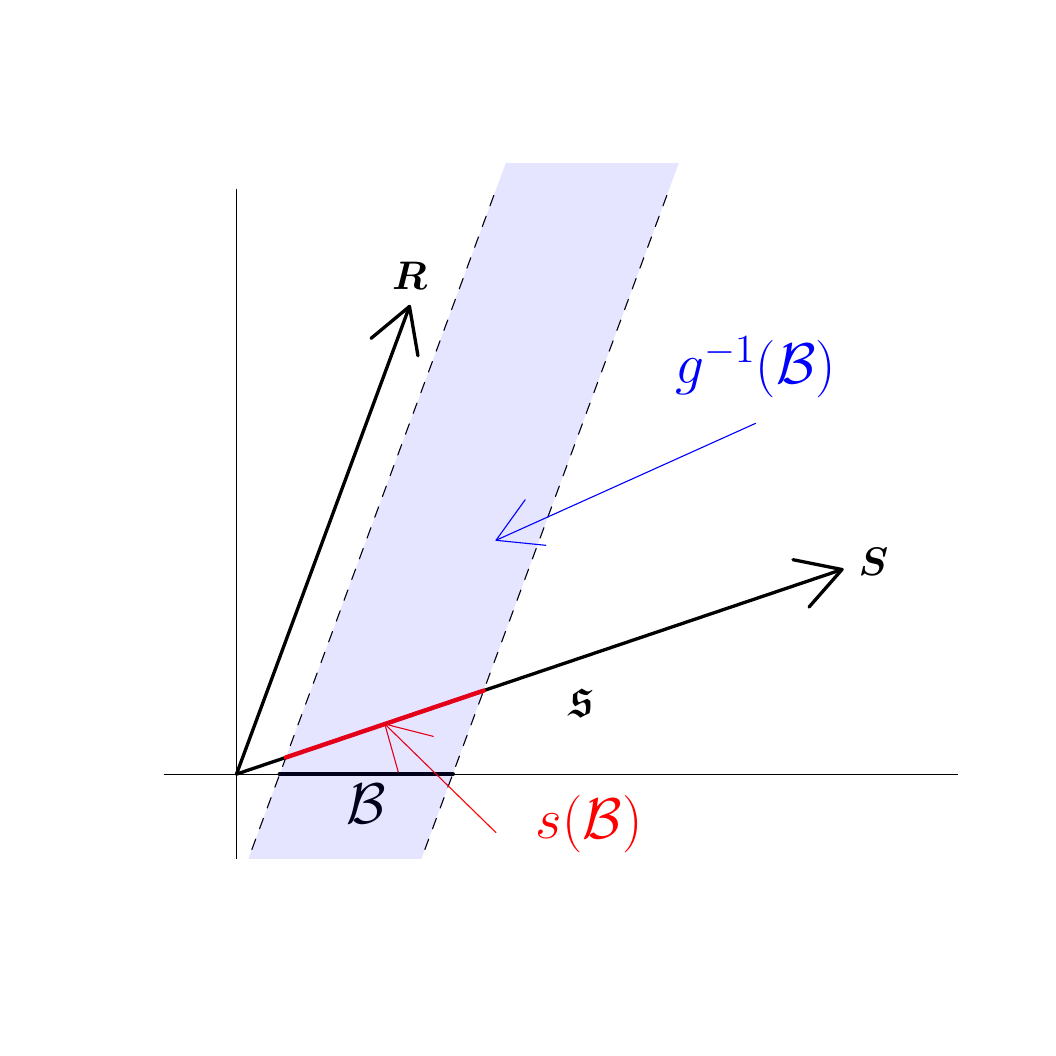
\begin{tikzpicture}[x=1pt,y=1pt]
\definecolor{fillColor}{RGB}{255,255,255}
\path[use as bounding box,fill=fillColor,fill opacity=0.00] (0,0) rectangle (361.35,361.35);
\begin{scope}
\path[clip] ( 49.20, 61.20) rectangle (336.15,312.15);
\definecolor{drawColor}{RGB}{0,0,0}

\path[draw=drawColor,line width= 0.4pt,line join=round,line cap=round] ( 75.46, 49.37) --
	( 75.46,302.86);

\path[draw=drawColor,line width= 0.4pt,line join=round,line cap=round] ( 12.94, 91.62) --
	(361.35, 91.62);

\path[draw=drawColor,line width= 1.2pt,line join=round,line cap=round] ( 75.46, 91.62) -- (294.26,165.55);

\path[draw=drawColor,line width= 1.2pt,line join=round,line cap=round] (282.33,151.98) --
	(294.26,165.55) --
	(276.55,169.10);

\node[text=drawColor,anchor=base west,inner sep=0pt, outer sep=0pt, scale=  1.00] at (300.26,163.26) {{\Large ${\bm S}$}};

\node[text=drawColor,anchor=base,inner sep=0pt, outer sep=0pt, scale=  1.00] at (200.49,112.53) {{\huge $\mathfrak{s}$}};

\path[draw=drawColor,line width= 1.2pt,line join=round,line cap=round] ( 75.46, 91.62) -- (137.97,260.61);

\path[draw=drawColor,line width= 1.2pt,line join=round,line cap=round] (141.02,242.80) --
	(137.97,260.61) --
	(124.07,249.07);

\node[text=drawColor,anchor=base,inner sep=0pt, outer sep=0pt, scale=  1.00] at (137.97,266.61) {{\Large ${\bm R}$}};

\path[draw=drawColor,line width= 0.4pt,dash pattern=on 4pt off 4pt ,line join=round,line cap=round] ( 75.46, 49.37) --
	(169.23,302.86);

\path[draw=drawColor,line width= 0.4pt,dash pattern=on 4pt off 4pt ,line join=round,line cap=round] (137.97, 49.37) --
	(231.75,302.86);

\path[draw=drawColor,line width= 1.6pt,line join=round,line cap=round] ( 91.09, 91.62) --
	(153.60, 91.62);

\node[text=drawColor,anchor=base,inner sep=0pt, outer sep=0pt, scale=  1.00] at (122.34, 73.88) {{\huge $\mathcal{B}$}};
\definecolor{drawColor}{RGB}{255,0,0}

\path[draw=drawColor,line width= 1.6pt,line join=round,line cap=round] ( 93.32, 97.65) --
	(164.77,121.79);
\definecolor{drawColor}{RGB}{0,0,0}

\node[text=drawColor,anchor=base west,inner sep=0pt, outer sep=0pt, scale=  1.00] at (183.63, 68.20) {{\huge $\color{red}{s(\mathcal{B})}$}};
\definecolor{drawColor}{RGB}{255,0,0}

\path[draw=drawColor,line width= 0.4pt,line join=round,line cap=round] (169.23, 70.49) -- (129.04,109.72);

\path[draw=drawColor,line width= 0.4pt,line join=round,line cap=round] (146.55,105.26) --
	(129.04,109.72) --
	(133.93, 92.33);
\definecolor{fillColor}{RGB}{0,0,255}

\path[fill=fillColor,fill opacity=0.10] ( 59.83,  7.12) --
	(122.34,  7.12) --
	(247.38,345.10) --
	(184.86,345.10) --
	cycle;
\definecolor{drawColor}{RGB}{0,0,255}

\node[text=drawColor,anchor=base,inner sep=0pt, outer sep=0pt, scale=  1.00] at (263.01,232.76) {{\huge $\color{blue}{g^{-1}(\mathcal{B}})$}};

\path[draw=drawColor,line width= 0.4pt,line join=round,line cap=round] (263.01,218.36) -- (169.23,176.11);

\path[draw=drawColor,line width= 0.4pt,line join=round,line cap=round] (179.79,190.78) --
	(169.23,176.11) --
	(187.21,174.30);
\end{scope}
\end{tikzpicture}
%\caption{a caption}
%\end{document}

	\caption{Summary of probabilistic forecast reconciliation. The probability that $\bm{y}_{t+h}$ lies in the red line segment under the reconciled probabilistic forecast is defined to be equal to the probability that $\bm{y}_{t+h}$ lies in the shaded blue area under the unreconciled probabilistic forecast. Note that since the smallest possible hierarchy involves three dimensions, this figure is only a schematic.}\label{fig:probfr_sch}
\end{figure}


\section{Parametric reconciliation} \label{sec:ParamRecon}

Recall that when $s\circ g$ is a projection, the case of point forecast reconciliation can be broken down into three steps. In what follows we drop the subscript $t+h$ from conditional forecasts for brevity.
\begin{compactenum}
	\item $\hat{\bm{y}}$ is transformed into coordinates $\tilde{\bm{b}}$ and $\tilde{\bm{a}}$ via a change of basis.
	\item $\tilde{\bm{a}}$ is discarded and $\tilde{\bm{b}}$ are kept as the bottom-level reconciled forecasts.
	\item Reconciled forecasts for the entire hierarchy are recovered via $\tilde{\bm{y}}=\bm{S}\tilde{\bm{b}}$.
\end{compactenum}

We now outline the analogous steps for probabilistic forecasts when predictive densities are available.

While $\hat{\nu}$ is a probability measure for an $n$-vector $\hat{\bm{y}}$, probability statements in terms of a different coordinate system can be made via an appropriate change of basis. Letting $f(.)$ be generic notation for a probability density function, and following the notation from point forecast reconciliation where $\hat{\bm{y}}=\bm{S}\tilde{\bm{b}}+\bm{R}\tilde{\bm{a}}$, we obtain
\begin{equation}
f(\hat{\bm{y}})=f(\bm{S}\tilde{\bm{b}}+\bm{R}\tilde{\bm{a}})|(\bm{S}~\bm{R})|
\end{equation}
The expression $\hat{\nu}(g^{-1}(\mathcal{B}))$ in Definition~\ref{def:reconprob} is equivalent to the probability statement $\text{Pr}(\hat{\bm{y}}\in g^{-1}(\mathcal{B}))$. After the change of basis, this is equivalent to $\text{Pr}(\tilde{\bm{b}}\in \mathcal{B})$, which implies
\begin{align}
	\text{Pr}(\hat{\bm{y}}\in g^{-1}(\mathcal{B}))&=\int\limits_{g^{-1}(\mathcal{B})}f(\hat{\bm{y}})d\hat{\bm{y}}\\
	&=\int\limits_{\mathcal{B}}\int f(\bm{S}\tilde{\bm{b}}
	+\bm{R}\tilde{\bm{a}})|(\bm{S}~\bm{R})|d\tilde{\bm{a}}d\tilde{\bm{b}}.
\end{align}
After integrating out over $\tilde{\bm{a}}$, a step analogous to setting $\tilde{\bm{a}}=0$ for point forecasting, we obtain an expression that gives the probability that the reconciled bottom-level series lies in the region $\mathcal{B}$. This corresponds to $\nu(\mathcal{B})$ in Definition~\ref{def:reconprob}. To make a valid probability statement about the entire hierarchy we simply use the bottom-level probabilistic forecasts together with Definition~\ref{def:cohprob}.

\subsubsection*{Example: Gaussian Distributions}

Suppose an unreconciled probabilistic forecast is Gaussian with mean $\hat{\bm{\mu}}$ and variance-covariance matrix $\hat{\bm{\Sigma}}$. Let the unreconciled density be given by
\begin{equation}
f(\hat{\bm{y}})=(2\pi)^{-n/2}|\hat{\bm{\Sigma}}|^{-1/2}\exp\left\{-\frac{1}{2}\left[(\hat{\bm{y}}-\hat{\bm{\mu}})'\hat{\bm{\Sigma}}^{-1}(\hat{\bm{y}}-\hat{\bm{\mu}})\right]\right\}.
\end{equation}
In an alternative basis,
\begin{equation}
f(\tilde{\bm{b}},\tilde{\bm{a}})=(2\pi)^{-\frac{n}{2}}\Big|\hat{\bm{\Sigma}}\Big|^{-\frac{1}{2}}\Big|(\bm{S} ~  \bm{R})\Big|\exp\{-\frac{1}{2}q\}\,,
\end{equation}
where
\begin{equation}
q=(\bm{S}\tilde{\bm{b}}+\bm{R}\tilde{\bm{a}}-\hat{\bm{\mu}})' \hat{\bm{\Sigma}}^{-1}(\bm{S}\tilde{\bm{b}}+\bm{R}\tilde{\bm{a}}-\hat{\bm{\mu}}).
\end{equation}
The quadratic form $q$ can be rearranged as
\begin{align*}
	q& =
	\left((\bm{S} ~  \bm{R})\bt-\hat{\bm{\mu}}\right)' \hat{\bm{\Sigma}}^{-1}\left((\bm{S} ~ \bm{R})\bt-\hat{\bm{\mu}}\right),\\
	& =
	\left(\bt-(\bm{S} ~ \bm{R})^{-1}\hat{\bm{\mu}}\right)' \Big[(\bm{S}  \bm{R})^{-1}\hat{\bm{\Sigma}}\left((\bm{S} ~ \bm{R})^{-1}\right)'\Big]^{-1}
	\left(\bt-(\bm{S} ~ \bm{R})^{-1}\hat{\bm{\mu}}\right)\,.
\end{align*}
Recall that
\[
(\bm{S} ~ \bm{R})^{-1} =
\begin{pmatrix}(\bm{R}'_\bot \bm{S})^{-1}\bm{R}'_\bot  \\ (\bm{S}'_\bot \bm{R})^{-1}\bm{S}'_\bot \end{pmatrix} :=
\begin{pmatrix}
\bm{G} \\\bm{H}
\end{pmatrix}\,.
\]
Then $q$ can be rearranged further as
\begin{align*}
	q& =%\frac{1}{(2\pi)^{\frac{n}{2}}\Big|\hat{\bm{\Sigma}}_{t+h}\Big|^{\frac{1}{2}}\Big|\PQ \Big|}
	%\exp \Big\{-\frac{1}{2}
	\left[\bt-\PQ\hat{\bm{\mu}}\right]'%\\[-0.5cm]
	\left[\PQ\hat{\bm{\Sigma}}\PQ'\right]^{-1}\left[\bt-\PQ\hat{\bm{\mu}}\right] %\Big\},
	\\[0.5cm]
	& =%\frac{1}{(2\pi)^{\frac{n}{2}}\Big|\PQ\hat{\bm{\Sigma}_{t+h}}\PQ'\Big|^{\frac{1}{2}}}
	%\exp \Big\{-\frac{1}{2}
	\begin{pmatrix}\tilde{\bm{b}} - \bm{G}\hat{\bm{\mu}}\\ \tilde{\bm{a}}- \bm{H}\hat{\bm{\mu}}\end{pmatrix}' %&\\[-0.5cm]
	%& \hspace*{7cm}
	\left[\PQ\hat{\bm{\Sigma}}\PQ'\right]^{-1}\begin{pmatrix}\tilde{\bm{b}} - \bm{G}\hat{\bm{\mu}}\\ \tilde{\bm{a}}- \bm{H}\hat{\bm{\mu}}\end{pmatrix}. %\Big\}.
\end{align*}
%Since $\Big[\PQ\hat{\bm{\Sigma}_{t+h}}\PQ'\Big] = \begin{pmatrix}
%\bm{P}\hat{\bm{\Sigma}_{t+h}}\bm{P}' & \bm{P}\hat{\bm{\Sigma}_{t+h}}\bm{Q}'
%\bm{Q}\hat{\bm{\Sigma}_{t+h}}\bm{P}' & \bm{Q}\hat{\bm{\Sigma}_{t+h}}\bm{Q}'
%\end{pmatrix}$ we have

Similar manipulations on the determinant of the covariance matrix lead to the following expression for the density:
\begin{align*}
	f(\tilde{\bm{b}},\tilde{\bm{a}})&
	=(2\pi)^{-\frac{n}{2}}\left|
	\begin{pmatrix}
		\bm{G}\hat{\bm{\Sigma}}\bm{G}' & \bm{G}\hat{\bm{\Sigma}}\bm{H}' \\
		\bm{H}\hat{\bm{\Sigma}}\bm{G}' & \bm{H}\hat{\bm{\Sigma}}\bm{H}'
	\end{pmatrix}
	\right|^{-\frac{1}{2}}
	\exp \left\{-\frac{1}{2} \begin{pmatrix}\tilde{\bm{b}} - \bm{G}\hat{\bm{\mu}}\\ \tilde{\bm{a}}- \bm{H}\hat{\bm{\mu}}\end{pmatrix}'\right.\\
	&\hspace*{7cm}
	\left.\begin{pmatrix}
		\bm{G}\hat{\bm{\Sigma}}\bm{G}' & \bm{G}\hat{\bm{\Sigma}}\bm{H}' \\
		\bm{H}\hat{\bm{\Sigma}}\bm{G}' & \bm{H}\hat{\bm{\Sigma}}\bm{H}'
	\end{pmatrix}^{-1}
	\begin{pmatrix}\tilde{\bm{b}} - \bm{G}\hat{\bm{\mu}}\\ \tilde{\bm{a}}- \bm{H}\hat{\bm{\mu}}\end{pmatrix} \right\}.
\end{align*}
Marginalising out $\tilde{\bm{a}}$ leads to the following bottom-level reconciled forecasts:
\begin{equation}\label{ex:2.1}
f(\tilde{\bm{b}})=(2\pi)^{-\frac{m}{2}}\Big|\bm{G}\hat{\bm{\Sigma}}\bm{G}'\Big|^{\frac{1}{2}}
\exp \Big\{-\frac{1}{2} (\tilde{\bm{b}} - \bm{G}\hat{\bm{\mu}})' (\bm{G}\hat{\bm{\Sigma}}\bm{G}')^{-1}(\tilde{\bm{b}} - \bm{G}\hat{\bm{\mu}}) \Big\}.
\end{equation}

%Equation \eqref{ex:2.1} implies $\tilde{\bm{b}}_{t+h} \sim \mathcal{N}(\bm{P}\hat{\bm{\mu}}_{t+h}, \bm{P}\hat{\bm{\Sigma}}_{t+h}\bm{P}')$, where $\bm{P} = (\bm{R}'_\bot \bm{S})^{-1}\bm{R}'_\bot$. Then from \eqref{4.7} it follows that
%\begin{equation}\label{eq:gaussianreconciled}
%\tilde{\bm{f}}(\tilde{\bm{y}}_{t+h})=\tilde{\bm{f}}(\bm{S}\tilde{\bm{b}}_{t+h}).
%\end{equation}
This implies that the reconciled probabilistic forecast for the bottom-level series is $\tilde{\bm{b}} \sim \mathcal{N}(\bm{G}\hat{\bm{\mu}}, \bm{G}\hat{\bm{\Sigma}}\bm{G}')$. The reconciled probabilistic forecasts for the whole hierarchy follow a degenerate Gaussian distribution with mean $\bm{SG}\hat{\bm{\mu}}$ and rank deficient covariance matrix $\bm{SG}\hat{\bm{\Sigma}}\bm{G}'\bm{S}'$.



\subsection{Elliptical distributions}

We now show that the true predictive distribution can be recovered for elliptical distributions by linear reconciliation via pre-multiplication and translation respectively by a matrix we denote ${\bm G}_{opt}$ and vector we denote ${\bm d}_{opt}$. Here, for any square matrix $\bm{C}$, $\bm{C}^{1/2}$ and $\bm{C}^{-1/2}$ are defined to satisfy $\bm{C}^{1/2}(\bm{C}^{1/2})'=\bm{C}$ and $\bm{C}^{-1/2}(\bm{C}^{-1/2})'=\bm{C}^{-1}$, for example $\bm{C}^{1/2}$ may be obtained via the Cholesky or eigenvalue decompositions.

\begin{theo}[Reconciliation for Elliptical Distributions]
	Let an unreconciled probabilistic forecast come from the elliptical class with location parameter $\hat{\bm{\mu}}$ and scale matrix $\hat{\bm{\Sigma}}$. Let the true predictive distribution of $\bm{y}$ also belong to the elliptical class with location parameter $\bm{\mu}$ and scale matrix $\bm{\Sigma}$. Then the linear reconciliation mapping $g(\breve{\bm{y}})=\bm{G}_{opt}\breve{\bm{y}}+\bm{d}_{opt}$ with $\bm{G}_{opt}={\bm{a}}\hat{\bm\Sigma}^{-1/2}$ and $\bm{d}_{opt}=\bm{\mu}-\bm{S}\bm{G}_{opt}\hat{\bm{\mu}}$ recovers the true predictive density where ${\bm{a}}$ is any $m\times n$ matrix such that ${\bm{a}}{\bm{a}}'=\bm{\Omega}$ and $\bm{\Omega}$ is a sub-matrix of $\bm{\Sigma}$ corresponding to the bottom-level series.
\end{theo}

\begin{proof}
	Since elliptical distributions are closed under affine transformations, and are closed under marginalisation, reconciliation of an elliptical distribution yields an elliptical distribution (although the unreconciled and reconciled distributions may be different members of the class of elliptical distributions). The scale matrix of the reconciled forecast is given by $\bm{S}\bm{G}_{opt}\hat{\bm{\Sigma}}\bm{G}_{opt}'\bm{S}'$, while the location matrix is given by $\bm{S}\bm{G}_{opt}\hat{\bm{\mu}}+\bm{d}_{opt}$. The reconciled scale matrix is
	\[
	\tilde{\bm{\Sigma}}_{opt}
	= \bm{S}{\bm{a}}\hat{\bm\Sigma}^{-1/2}\hat{\bm{\Sigma}}\left(\hat{\bm\Sigma}^{-1/2}\right)'{\bm{a}}'\bm{S}'
	= \bm{S}\bm{\Omega}\bm{S}'
	= \bm{\Sigma}.
	\]
	For the choices of $\bm{G}_{opt}$ and $\bm{d}_{opt}$ given above, the reconciled location vector is
	\[
	\tilde{\bm{\mu}}_{opt}= \bm{S}\bm{G}_{opt}\hat{\bm{\mu}}+\bm{\mu}-\bm{S}\bm{G}_{opt}\hat{\bm{\mu}}
	= \bm{\mu}.
	\]
\end{proof}

A number of insights can be drawn from this theorem. First, although a linear function $g(.)$ can be used to recover the true predictive in the elliptical case, the same does not hold in general. Second, $g(.)$ is not, in general, a projection matrix. The conditions for which a the true predictive density can be recovered by a projection are given below.

\begin{theo}[True predictive via projection]
	Assume that the true predictive distribution is elliptical with location $\bm{\mu}$ and scale $\bm{\Sigma}$. Consider reconciliation via a projection $g(\bm{y})=(\bm{R}'_{\perp}\bm{S})^{-1}\bm{R}'_{\perp}\bm{y}$. The true predictive distribution can be recovered via reconciliation of an elliptical distribution with location $\hat{\bm{\mu}}$ and scale $\hat{\bm{\Sigma}}$ when the following conditions hold:
	\begin{align}
		sp(\hat{\bm\mu}-\bm{\mu})&\subset sp(\bm{R})\\
		sp(\hat{\bm{\Sigma}}^{1/2}-\bm{\Sigma}^{1/2})&\subset sp(\bm{R})\\
	\end{align}
\end{theo}

\begin{proof}
	The reconciled location vector will be given by
	\begin{align*}
		\tilde{\bm{\mu}}&=\bm{S}(\bm{R}'_{\perp}\bm{S})^{-1}\bm{R}'_{\perp}\hat{\bm{\mu}}\\
		&=\bm{S}(\bm{R}'_{\perp}\bm{S})^{-1}\bm{R}'_{\perp}\left(\hat{\bm{\mu}}+\bm{\mu}-\bm{\mu}\right)\\
		&=\bm{S}(\bm{R}'_{\perp}\bm{S})^{-1}\bm{R}'_{\perp}\bm{\mu}+\bm{S}(\bm{R}'_{\perp}\bm{S})^{-1}\bm{R}'_{\perp}\left(\hat{\bm{\mu}}-\bm{\mu}\right).
	\end{align*}
	Since $\bm{S}(\bm{R}'_{\perp}\bm{S})^{-1}\bm{R}'_{\perp}$ is a projection onto $\mathfrak{s}$ and $\bm{\mu}\in\mathfrak{s}$, the first term simplifies to $\bm{\mu}$. If $\bm{\mu}-\hat{\bm{\mu}}$ lies in the span of $\bm{R}$, then multiplication by $\bm{R}'_{\perp}$ reduces the second term to $\bm{0}$. By a similar argument it can be shown that $\tilde{\bm{\Sigma}}^{1/2}=\bm{\Sigma}^{1/2}$. The closure property of elliptical distributions under affine transformations ensures that the full true predictive distribution can be recovered.
\end{proof}

Although these conditions will rarely hold in practice and only apply to a limited class of distributions, they do provide some insight into selecting a projection for reconciliation. If the value of $\hat{\bm{\mu}}$ were equi-probable in all directions, then a projection orthogonal to $\mathfrak{s}$ would be a sensible choice for $\bm{R}$ since it would in some sense represent a `median' direction for $\bm{\mu}-\hat{\bm{\mu}}$. However, the one-step-ahead in-sample errors are usually correlated suggesting that $\hat{\bm{\mu}}$ is more likely to fall in some directions than others. Therefore an orthogonal projection after transformation by the inverse of the one-step-ahead in-sample error covariance matrix may be more intuitively appealing. This is exactly what the MinT projection provides, and we demonstrate this in a simulation setting in the following subsection.



%However, these expressions do provide some insight on why some choices for $\bm{G}$ in the point forecast reconciliation literature may also work well for probabilistic forecasts. To illustrate, first rearrange the equation for the optimal value of $\bm{G}_{opt}={\bm\Omega}^{1/2}\hat{\bm\Sigma}^{-1/2}$ as ${\bm\Omega}^{1/2}=\bm{G}_{opt}\hat{\bm\Sigma}^{1/2}$. For arbitrary $\bm{G}\hat{\bm\Sigma}^{1/2}$ is an approximation for ${\bm\Omega}^{1/2}$. This approximation has similarities with the way bottom-level estimates are produced for point forecast reconciliation. Rather than mapping a vector of point forecasts to reconcilied bottom-level forecasts, the columns of $\hat{\bm\Sigma}^{1/2}$ are mapped to an approximation of the columns of ${\bm\Omega}^{1/2}$. The value for $\tilde{\bm{\mu}}_{opt}$ includes a projection of $\hat{\bm{\mu}}$ onto $\mathfrak{s}$. While it is infeasible to obtain the translation $\bm{d}$, it is worthwhile noting that this measures the difference between the reconciled mean and true mean.

\section{Sample based solution: A novel non-parametric bootstrap approach}\label{sec:non-para}

Often in practice we come across hierarchical time series that have high level of disaggregation and/or contain even discrete data. For these time series, parametric distributional assumptions are misleading. An alternative for such cases is to apply non-parametric approaches. Hence we propose a novel non-parametric bootstrap based approach for obtaining coherent probabilistic forecasts.

Our proposed method initially involves obtaining probabilistic forecasts without considering the aggregation constraints. These incoherent probabilistic forecasts are then reconciled to make them coherent. We first focus on the methodology for obtaining base forecasts.

\subsection{Incoherent probabilistic forecasts} \label{Subsec:Incoherent_samplePaths}
First we fit appropriate univariate models for each series in the hierarchy based on the training data $\bm{y}_{1:T}$. We then compute 1-step-ahead training errors as $e_{i,t} = y_{i,t} - \hat{y}_{i,t}$ for $i=1,\dots,n$ and $t = 1,\dots,T$ where $\hat{y}_{i,t} = E(y_{i,t}|y_{i,1:t-1})$. The training errors are stored in a matrix $\bm{\Gamma}_{(T \times n)} = (\bm{e}_1,\dots,\bm{e}_T)'$ where $\bm{e}_t = (e_{1,t},\dots,e_{n,t})$ is stored in the same order as $\bm{y}_t$ for $t=1,\dots,T$. Next we block bootstrap a sample of size $H$ from $\bm{\Gamma_{(T \times n)}}$. That is, we randomly select $H$ consecutive rows from $\bm{\Gamma}$ and store in a matrix $\bm{\Gamma}^b_{(H \times n)} = (\bm{e}^b_1,\dots,\bm{e}^b_H)'$ and repeat this for $b = 1,\dots,B$.

Finally we generate the $h$-step-ahead future paths using the fitted univariate models conditioning on the past observations. We also incorporate the bootstrapped training errors as the error series for generating these future paths. By doing so we implicitly model the contemporaneous correlation structure of the hierarchy. Further the use of consecutive (block) training errors will ensure that the serial correlation of the series is accounted for. To explain this process more explicitly consider the following example.

\noindent
\textbf{Example:}
Suppose we fit an $ARMA(p,q)$ model for the $i^\text{th}$ series of the hierarchy. i.e.,
\begin{align*}
	y_{i,t} &= \alpha_1y_{i,t-1} + \alpha_2y_{i,t-2}+\dots+\alpha_py_{i,t-p} + \beta_1\epsilon_{i,t-1} + \beta_1\epsilon_{i,t-2}+\dots+\beta_q\epsilon_{i,t-q} + \epsilon_{i,t},\\
	y_{i,t} &= (\alpha_1 + \alpha_2L+\dots+\alpha_pL^{p-1})y_{i,t-1} + (\beta_1 + \beta_1L+\dots+\beta_qL^{q-1})\epsilon_{i,t-1} + \epsilon_{i,t}
\end{align*}
where $L$ is the usual lag operator. Then the $h$-step-ahead $b^\text{th}$ future path conditional on past information up to and including time $t$, for the $i^\text{th}$ series is produced as,
\begin{align*}
	\hat{y}^b_{i,t+h} &= (\hat{\alpha}_1 + \hat{\alpha}_2L +\dots+ \hat{\alpha}_pL^{p-1})y_{i,t+h-1} + (\hat{\beta}_1 + \hat{\beta}_1L+\dots+\hat{\beta}_qL^{q-1})\epsilon_{i,t+h-1} + e^b_{i,h}
\end{align*}
where, $e^b_{i,h}$ is the $(h\times i)^\text{th}$ element from $\bm{\Gamma}^b$,
\begin{equation*}
	y_{i,t+h-1} =
	\begin{cases}
		y_{i,1}:y_{i,T}       & \quad \text{for } t+h-1 \le T\\
		\hat{y}^b_{i,T+1}:\hat{y}^b_{i,T+h-1}  & \quad \text{for } t+h-1 > T
	\end{cases}
\end{equation*}
and
\begin{equation*}
	\epsilon_{i,t+h-1} =
	\begin{cases}
		\epsilon_{i,1}:\epsilon_{i,T}       & \quad \text{for } t+h-1 \le T\\
		e^b_{i,1}:e^b_{i,h-1}  & \quad \text{for } t+h-1 > T
	\end{cases}.
\end{equation*}

Once we obtain the $h$-step-ahead sample path for all $n$ series in the hierarchy, we stack them in the same order as $\hat{\bm{y}}_{t+h}$. Repeating the same process for $b = 1,\dots,B$ we obtain a set of $h$-step-ahead bootstrapped future paths of size $B$. We denote this as $\hat{\bm{\Upsilon}}_{T+h} = (\hat{\bm{y}}^1_{T+h},\dots,\hat{\bm{y}}^B_{T+h})'$ where the $b^\text{th}$ row of $\hat{\bm{\Upsilon}}_{T+h}$ represents the $h$-step-ahead $b^\text{th}$ sample path for all series in the hierarchy.

We note that $\hat{\bm{\Upsilon}}_{T+h}$ is an empirical sample from the incoherent probability distribution of the hierarchy. Since the aggregation constraints are not imposed while generating $\hat{\bm{\Upsilon}}_{T+h}$, it is very unlikely that they lie on the coherent subspace. Thus it requires reconciliation to which we now turn our attention.

\subsection{Reconciliation of incoherent future paths}

To reconcile the incoherent sample paths, we follow the definition of reconciliation. We project each sample path in $\hat{\bm{\Upsilon}}_{T+h}$ to the coherent subspace via the projection $\bm{SG}$. i.e. for any $\bm{G}$ we can write,

\begin{equation} \label{eq:sampleRecon_1}
\tilde{\bm{y}}_{T+h}^b = \bm{SG}\hat{\bm{y}}_{T+h}^b,
\end{equation}
consequently we have,

\begin{equation} \label{eq:sampleRecon_2}
\tilde{\bm{\Upsilon}}'_{T+h} = \bm{SG}\hat{\bm{\Upsilon}}'_{T+h},
\end{equation}

where, each row in $\tilde{\bm{\Upsilon}}_{T+h}$ represent a single reconciled sample path. Further $\tilde{\bm{\Upsilon}}_{T+h}$ form an empirical sample from the reconciled forecast distribution of the hierarchy. Any $\bm{G}$ matrix introduced in point forecast reconciliation (also given in Table \ref{table:ReconMethods}) can be used for this sample path reconciliation. However, in the following subsection we discuss a method to find $\bm{G}$ that is optimal for probabilistic forecasts with respect to a proper scoring rule.

\subsection{Optimal reconciliation of incoherent future paths}\label{subsec:Optimal_recon}

Let us now propose to find an optimal $\bm{G}$ for reconciling future paths by minimising a proper multivariate scoring rule. The respective objective function can be written as,

\begin{equation} \label{eq:Obj_func_1}
\operatornamewithlimits{argmin}_{\bm{G}_h} \quad \E_{\bm{Q}}[S(\bm{SG}_h\hat{\bm{\Upsilon}}'_{T+h}, \bm{y}_{T+h})],
\end{equation}
where $S$ is a proper scoring rule that follows equation (\ref{eq:prop_score}). We use the subscript $h$ on $\bm{G}$ to emphasise distinct $\bm{G}$ matrices for different forecast horizons. Recall that the energy score given in equation (\ref{eq:Energy_score}) is a proper scoring rule. Let $\alpha = 1$ and following equation (\ref{eq:ES_with_MCSamples}) we can write,

\begin{equation}\label{eq:ES_with_Samplespaths}
\text{ES}(\bm{SG}_h\hat{\bm{\Upsilon}}'_{T+h}, \bm{y}_{T+h}) \approx \frac{1}{B}\sum_{b=1}^{B}||\bm{SG}_h\hat{\bm{y}}_{T+h,j}^b -\bm{y}_{T+h}||-\frac{1}{2(B-1)}\sum_{b=1}^{B-1}||\bm{SG}_h(\hat{\bm{y}}_{T+h,j}^b -\hat{\bm{y}}_{T+h,j}^{b+1})||.
\end{equation}
where $B$ is the empirical sample size from the coherent forecast distribution. Now we can rewrite the objective function in (\ref{eq:Obj_func_1}) as,

\begin{equation}\label{eq:Obj_func_2}
\operatornamewithlimits{argmin}_{\bm{G}} \frac{1}{N}\sum_{j=1}^{N}\left\{\frac{1}{B}\sum_{b=1}^{B}||\bm{SG}_h\bm{y}_{T+h,j}^b -\bm{y}_{T+h,j}||-\frac{1}{2(B-1)}\sum_{b=1}^{B-1}||\bm{SG}_h(\bm{y}_{T+h,j}^b -\bm{y}_{T+h,j}^{b+1})||\right\}
\end{equation}
where, the expectation $E_{\bm{Q}}$ over true forecast distribution $\bm{Q}$ is approximated through the sample mean over $\{\text{ES}(\bm{SG}_h\hat{\bm{\Upsilon}}'_{T+h,1}, \bm{y}_{T+h,1}),\dots,\text{ES}(\bm{SG}_h\hat{\bm{\Upsilon}}'_{T+h,N}, \bm{y}_{T+h,N})\}$.
We can use numerical optimization methods to estimate the matrix $\bm{G}_h$ that minimises the above objective function and thus obtain the optimally reconciled future paths.

We have also considered different parameterisation methods for estimation optimal $\bm{G}_h$. This was discussed in Section \ref{Appen:ReparaG} in Appendix. 

%and the results are presented in Section \ref{Appen:ReparaG_sim} in Appendix. We note that the 


%We propose to find an optimal $\bm{G}$ for reconciling future paths by minimizing a proper scoring rule defined in \ref{eq:prop_score}. Scoring rule is a numerical value $Sc(\breve{\bm{Y}},\bm{y})$ assign to each pair $(\breve{\bm{Y}},\bm{y})$, where $\breve{\bm{Y}}$ is a $n$-dimensional random vector from the forecast distribution $\breve{\bm{F}}$ and $\bm{y}$ is a realization. A proper scoring rule is defined as,
%\begin{equation}\label{eq:(2.3)}
%\E_{\bm{G}}[Sc(\bm{Y},\bm{y})] \le \E_{\bm{G}}[Sc(\breve{\bm{Y}},\bm{y})],
%\end{equation}
%where $\bm{Y}$ is a random variable from the true distribution $\bm{G}$ \citep{Gneiting2014}.
%
%Thus the minimization problem for finding the optimal $\bm{R}_\bot$ will be
%\begin{equation}
%\operatornamewithlimits{argmin}_{\bm{R}'_\bot} \quad \E_{\bm{G}}[Sc(\bm{S}(\bm{R}'_\bot \bm{S})^{-1}\bm{R}'_\bot\bm{y}_{t+h}^b, \bm{y}_{t+h})].
%\end{equation}


%We generate data with a sample size of $T=501$. Univariate ARIMA models are selected for each series using the \textit{auto.arima} function in the \textit{forecast} package \citep{hyndman2017forecasting} in R \citep{Rcore}. The same package was used to fit each series independently using the first 500 observations, and evaluate 1-step ahead base (incoherent) probabilistic forecasts. These were then reconciled using different projections summarised in Table~\ref{table:2}. This process was replicated using $1000$ different data sets from the same data generating processes.

%
%Table~\ref{table:3} summarizes the forecasting performance of unreconciled, bottom-up, OLS, WLS and two MinT reconciliation methods using log score, energy score and variogram score. In all cases skill scores are calculated with the bottom-up method as reference. All log scores are evaluated on the basis of bottom-level series only, however these only differ from the log scores for the full hierarchy by a fixed constant. The cell for log score of unreconciled forecasts is left blank since the log score is not proper in this context. Overall, the MinT methods provide the best performance irrespective of the scoring rule, and all methods that reconcile using information at all levels of the forecast improve upon unreconciled forecasts. Bottom-up forecasts perform even worse than unreconciled forecasts in some cases.
%
%Tables~\ref{table:4} and~\ref{table:5} break down the forecasting performance of different reconciliation methods by considering univariate scores on each individual margin. Tables~\ref{table:4} summarises results for the top and middle-level, Table~\ref{table:5} does the same for bottom-level. The log score and CRPS are considered, while skill scores are computed with the unreconciled forecast as a reference. When broken down in this fashion, the methods based on MinT perform best for all series and always outperform bottom-up and unreconciled forecasts.
%

\section{Evaluation of hierarchical probabilistic forecasts}\label{sec:evaluation}

The necessary final step in hierarchical forecasting is to make sure that our forecast distributions are accurate. In general, forecasters prefer to maximize the sharpness of the forecast distribution subject to calibration \citep{Gneiting2014}. Therefore the probabilistic forecasts should be evaluated with respect to these two properties.

Calibration refers to the statistical compatibility between probabilistic forecasts and realizations. In other words, random draws from a perfectly calibrated forecast distribution should be equivalent in distribution to the realizations. On the other hand, sharpness refers to the spread or the concentration of the predictive distributions and it is a property of the forecasts only. The more concentrated the forecast distributions, the sharper the forecasts \citep{Gneiting2008}. However, independently assessing the calibration and sharpness will not help to properly evaluate the probabilistic forecasts. Therefore we need to assess these properties simultaneously using scoring rules.

Scoring rules are summary measures obtained based on the relationship between the forecast distributions and the realizations. In some studies, researchers take the scoring rules to be positively oriented, in which case the scores should be maximized \citep{Gneiting2007}. However, scoring rules have also been defined to be negatively oriented, and then the scores should be minimized \citep{Gneiting2014}. We follow the latter convention here.

Let $P$ be a forecast distribution and let $Q$ be the true data generating process respectively. Furthermore let $\omega$ be a realization from $Q$. Then a scoring rule is a function $S(P,\omega)$ that maps $P,\omega$ to $\mathbb{R}$. It is a ``proper'' scoring rule if
\begin{equation}\label{eq:prop_score}
\E_{\bm{Q}}[S(Q,\omega)] \le \E_{\bm{Q}}[S(P,\omega)] ,
\end{equation}
where $\E_{Q}[S(P,\omega)]$ is the expected score under the true distribution $Q$ \citep{Gneiting2008, Gneiting2014}. When this inequality is strict, the scoring rule is said to be strictly proper.

In the context of probabilistic forecast reconciliation there could be two motivations for using scoring rules. The first is to compare unreconciled densities to reconciled densities. Reconciliation itself is a valuable goal since it can be important in aligning decision making across, for example, different units of an enterprise. In the point forecasting literature, forecast reconciliation has also been shown to improve forecast performance \citep{AthEtAl2017, WicEtAl2019}. It will be worthwhile to see whether the same holds in the probabilistic forecasting case. The second motivation for using scoring rules is to compare two or more sets of reconciled probabilistic forecasts to one another. The objective here is to evaluate which reconciliation mapping $g(.)$ works best in practice.

\subsection{Univariate scoring rules}

One way to evaluate hierarchical probabilistic forecasts is via the application of univariate scoring rules to each time series in the hierarchy. A summary can be taken of the expected scores across each margin, for example a mean or median. We consider two such scoring rules. The log score is given by the log density, in this case for each margin of the probabilistic forecast. The continuous rank probability score generalises mean square error and is given by
\begin{align} \label{eq:CRPS}
\text{CRPS}(\breve{F}_i,y_{i}) &=\int \left(\breve{F}_i(\breve{Y}_i)-\mathbb{1}(\breve{Y}_i<y_{i})\right)d\breve{Y}_i\\ &=\E_{\breve{Y}_i}|\breve{Y}_{i}-y_{i}| - \frac{1}{2}\E_{\breve{Y}_i}|\breve{Y}_{i}-\breve{Y}^*_{i}|\,,
\end{align}
where $\breve{F}_i$ is the cumulative distribution function of the $i^{\text{th}}$ margin of the probabilistic forecast, $\breve{Y}_i$ and $\breve{Y}^*_{i}$ are independent copies of a random variable with distribution $\breve{F}_i$, and $y_i$ is the outcome of the $i^{\text{th}}$ margin. The expectations in the second line can be approximated by Monte Carlo when a sample from the predictive distribution is available.

An advantage of this approach is that it allows the forecaster to separately evaluate different levels and individual series of the hierarchy to determine where the gains from reconciliation are greatest. For this reason this approach has been used in the limited literature on probabilistic forecasting for hierarchies \citep{BenTaieb2017, JeoEtAl2019} to date. A major shortcoming of this approach however, is that evaluating univariate scores on the margins does not account for the dependence in the hierarchy.

\subsection{Multivariate scoring rules}

While a number of alternative proper scoring rules are available for univariate forecasts, the multivariate case is somewhat more limited. Here we focus on three scoring rules: the log score (LS), the energy score (ES) and the variogram score (VS).

The log score can be approximated using a sample of values from the probabilistic forecast density \citep{Jordan2017}; however it is more commonly used when a parametric form for the density is available for the probabilistic forecast.

The energy score on the other hand can be defined in terms of the characteristic function of the probabilistic forecast, but the following representation in terms of expectations
\begin{equation}\label{eq:Energy_score}
\text{ES}(\breve{\bm{Y}}_{T+h},\bm{y}_{T+h}) =
\E_{\breve{\bm{Y}}}
||\breve{\bm{Y}}_{T+h}-\bm{y}_{T+h}||^\alpha -\frac{1}{2}\E_{\breve{\bm{Y}}}||\breve{\bm{Y}}_{T+h}-\breve{\bm{Y}}^*_{T+h}||^\alpha, \,\, \alpha \in (0,2]\,,
\end{equation}
lends itself to easy computation when samples from the probabilistic forecast are available and given as,
\begin{equation}\label{eq:ES_with_MCSamples}
\text{ES}(\breve{\bm{Y}}_{T+h},\bm{y}_{T+h}) \approx \frac{1}{M}\sum_{i=1}^{M}||\bm{SG}\breve{\bm{y}}_{T+h,i} -\bm{y}_{T+h}||-\frac{1}{2(M-1)}\sum_{i=1}^{M-1}||\bm{SG}(\breve{\bm{y}}_{T+h,i} -\breve{\bm{y}}_{T+h,i+1})||,
\end{equation}
where, $\breve{\bm{y}}_{T+h,i}$ is the $i^\text{th}$ Monte-Carlo sample from the forecast distribution. An interesting limiting case is where $\alpha=2$, where it can be easily shown that energy score simplifies to mean squared error around the mean of the predictive distribution. In this limiting case, the energy score is proper but not strictly proper. \citet{Pinson2013a} also argue that the energy score has low discriminative ability for incorrectly specified covariances, even though it discriminates the misspecified means well.

In contrast, \citet{SCHEUERER2015} have shown that the variogram score has a higher discrimination ability for misspecified means, variances and correlation structures than the energy score. When $\breve{\bm{y}}$ is a random variable from probabilistic forecast $\breve{F}$, the empirical variogram score is defined as
\begin{equation}
\text{VS}(\breve{F}, \bm{y}) = \displaystyle\sum_{i=1}^{n}\displaystyle\sum_{j=1}^{n}w_{ij}\left(|y_{i} - y_{j}|^p - E_{\breve{Y}_i,\breve{Y}_j} |\breve{Y}_{i}-\breve{Y}_{j}|^p\right)^2.
\end{equation}
\citet{SCHEUERER2015} recommend using $p=0.5$.



\subsubsection{Comparing unreconciled forecasts to reconciled forecasts}

For both reconciled and unreconciled densities it is possible to obtain a density from the probability measures defined in Section~\ref{sec:ProbForecasts}. Therefore it may seem sensible to compare unreconciled densities to reconciled densities on the basis of log score. However, the following theorem shows that using the log score may fail in the case of multivariate distributions with a degeneracy.

\begin{theo}[Impropriety of log score]\label{theo:logS_improp}
	When the true data generating process is coherent, then the log score is improper with respect to the class of incoherent measures.
\end{theo}

\begin{proof}
	Consider a rotated version of hierarchical time series, $\bm{z}_t=\bm{U}\bm{y}_t$, so that the first $m$ elements of $\bm{z}_t$ denoted $\bm{z}^{(1)}_t$ are unconstrained, while the remaining $n-m$ elements denoted $\bm{z}^{(2)}_t$ equal $0$ when the aggregation constraints hold. An example of the $n\times n$ $\bm{U}$ is the matrix of left singular vectors of $\bm{S}$.
	
	Consider the case where the true predictive density is $f_1(\bm{z}^{(1)}_t)\mathbb{1}\left(\bm{z}^{(2)}_t=\bm{0}\right)$, and we evaluate an incoherent density given by $f_1(\bm{z}^{(1)}_t)f_2(\bm{z}^{(2)}_t)$, where $f_2$ is highly concentrated around $0$ but still non-degenerate. For example, $f_2$ may be Gaussian with variance $\sigma^2{\bm{I}}$ with $\sigma^2 < (2\pi)^{-1}$. The log score under the true data generating process is
	\[
	LS\left(f,\bm{z}^{(1)}_t\right) = -\log f_1\left(\bm{z}^{(1)}_t\right),
	\]
	while that of the unreconciled density is
	\begin{align}
	LS\left(\hat{f},\bm{z}^{(1)}_t\right) &= -\log f_1(\bm{z}^{(1)}_t)- \log f_2(\bm{z}^{(1)}_t)\\
	&= -\log f_1(\bm{z}^{(1)}_t)+\frac{n-m}{2}\log(2\pi\sigma^2)\\
	&<-\log f_1(\bm{z}^{(1)}_t)=LS\left(f,\bm{z}^{(1)}_t\right).
	\end{align}
	After taking expectations $E\left[LS(f,f)\right] > E\left[LS(\hat{f},f)\right]$, violating the condition in Equation~\eqref{eq:prop_score} for a proper scoring rule.
\end{proof}

A similar issue also arises when discrete random variables are modelled as if they were continuous, an issue discussed in Section~4.1 of \citet{Gneiting2007}. This implies that the log score should be avoided when comparing reconciled and unreconciled probabilistic forecasts.

\subsubsection{Comparing reconciled forecasts to one another}

Coherent probabilistic forecasts can be completely characterised in terms of basis series; if a probabilistic forecast is available for the basis series, then a probabilistic forecast can be recovered for the entire hierarchy via Definition~\ref{def:cohprob}. This may suggest that it is adequate to merely compare two coherent forecasts to one another using the basis series only. We now show how this depends on the specific scoring rule used.

For the log score, suppose the coherent probabilistic forecast has density $f(\bm{b})$. The density for the full hierarchy is given by $f(\bm{y})=f(\bm{Sb})=f(\bm{b})J^{-1}$, where $J=\prod_{j=1}^{m}\lambda_j$ is a pseudo-determinant of the non-square matrix $\bm{S}$ and $\lambda_j$ are the non-zero singular values of $\bm{S}$. Therefore for any coherent density, the log score of the full hierarchy differs from the log score for the bottom-level series by the term $log(J)$. This term depends only on the structure of the hierarchy and is fixed across different reconciliation methods. Therefore if one method achieves a lower expected log score compared to an alternative method using the bottom-level series only, the same ordering is preserved when an assessment is made on the basis of the full hierarchy.

The same property does not hold for all scores in general. For example, the energy score can be expressed in terms of expectations of norms. In general, since norms are invariant under orthogonal rotations, the energy score is also invariant under orthogonal transformations \citep{Szekely2013,Gneiting2007}. In the context of two coherent forecasts, the same is true of a semi-orthogonal transformation from a lower dimensional basis series to the full hierarchy. However, when $\bm{S}$ is the usual summing matrix, it is not semi-orthogonal. Therefore the energy score computed on the bottom-level series will differ from the energy score computed using the full hierarchy and the ordering of different reconciliation methods may change depending on the basis series used. In this case we recommend computing the energy score using the full hierarchy. Although the discussion here is related to energy score, the same logic holds for other multivariate scores, for example the variogram score.

The properties of multivariate scoring rules in the context of evaluating reconciled probabilistic forecasts are summarised in Table~\ref{tab:prop}.

\begin{table}
	\caption{Summary of properties of scoring rules in the context of reconciled probabilistic forecasts.}
	\centering
	\begin{tabular}{rll}
		& Coherent v Incoherent &Coherent v Coherent\\
		\hline
		Log Score & Not proper & Ordering preserved if compared using\\ &&bottom-level only\\
		Energy/ & Proper & Full hierarchy should be used\\
		Variogram Score & Proper & Full hierarchy should be used\\
		\hline
	\end{tabular}
	
	\label{tab:prop}
\end{table}


\subsubsection{Skill scores}

To facilitate comparisons between different forecasting methods, we use skill scores \citep{Gneiting2007}. The skill score for a given forecast distribution $P$,  with reference to a forecast distribution $P_{ref}$, evaluated by a particular scoring rule $S()$, is calculated as, 

\begin{equation}
SS(P, \omega) = \frac{E_Q[S(P_{ref}, \omega)] - E_Q[S(P, \omega)]}{E_Q[S(P_{ref}, \omega)]}
\end{equation}

The skill score gives the percentage improvement of the preferred forecasting method relative to the reference method. A negative valued skill score indicates that a method is worse than the reference method, whereas any positive value indicates that the method is superior to the reference method. 


\section{Simulations}

We now present the simulation study carried-out to evaluate the performance of probabilistic forecasts in both parametric and non-parametric setting. Let us first discuss the data generating process.

\subsection{Data generating process (DGP)} \label{subsec:DGP}

The data generating process we consider is the hierarchy given in Figure \ref{fig:twoL-hier}, comprising two aggregation levels with four bottom-level series. Each bottom-level series will be generated first, and then summed to obtain the data for the upper-level series.

First $\{w_{AA,t},w_{AB,t},w_{BA,t},w_{BB,t}\}$ are generated from ARIMA$(p,d,q)$ processes, where $(p,q)$ and $d$ take integers from $\{1,2\}$ and $\{0,1\}$ respectively with equal probability. The parameters for the AR and MA components are randomly and uniformly generated from $[0.3,0.5]$ and $[0.3,0.7]$ respectively.
The errors driving the ARIMA processes were generated from Gaussian and non-Gaussian distributions separately. This will allow us to demonstrate the distinct impact of true DGP for parametric and non-parametric reconciliation approaches. 


\subsubsection*{Gaussian errors:}

Errors were jointly generated from a normal distribution, and denoted by $\{\varepsilon_{AA,t},\varepsilon_{AB,t},\varepsilon_{BA,t},\varepsilon_{BB,t}\} \overset{iid}{\sim} \mathcal{N}(\bm{0}, \bm{\Sigma})~\forall t$, where,


\begin{equation}\label{eq:SigmaGaussian}
\bm{\Sigma} =
\begin{pmatrix}
5.0 & 3.1 & 0.6 & 0.4 \\
3.1 & 4.0 & 0.9 & 1.4 \\
0.6 & 0.9 & 2.0 & 1.8 \\
0.4 & 1.4 & 1.8 & 3.0 \\
\end{pmatrix}\,.
\end{equation}


\subsubsection*{Non-Gaussian errors:}

Non-Gaussian errors were generated from a Gumbel copula model with beta margins. Using a copula model helps to impose a non-linear dependence structure among the series. A two dimensional Gumbel copula is given by,
\begin{equation*}
C_\theta(u_1, u_2) = exp\{-[(-ln(u_1))^\theta + (-ln(u_2))^\theta]^{1/\theta}\}.
\end{equation*}
We generate random variates $\{u_{AA}, u_{AB}\}$ from $C_{\theta=10}(.)$ and $\{u_{BA}, u_{BB}\}$ from $C_{\theta=8}(.)$ for series $\{AA, AB\}$ and $\{BA, BB\}$ respectively. Next we generate the errors, $\{\varepsilon_{AA}, \varepsilon_{AB}, \varepsilon_{BA}, \varepsilon_{BB}\}$ as the quantiles from beta distributions with shape parameters $\alpha = 1$ and $\beta = 3$ correspond to $\{u_{AA}, u_{AB}, u_{BA}, u_{BB}\}$.

%Although copulas go beyond the concepts of linear dependence, we will apply a Gaussian assumption to the data to investigate model misspecification. To give some idea of the covariance matrix of $\{\varepsilon_{AA}, \varepsilon_{AB}, \varepsilon_{BA}, \varepsilon_{BB}\}$, the sample estimate is,
%
%\begin{equation} \label{eq:SigmaNonGauss}
%\bm{\Sigma} = \begin{pmatrix}
%0.0388 & 0.0385 & 0.0010 & 0.0010\\
%0.0385 & 0.0390 & 0.0008 & 0.0008 \\
%0.0010 & 0.0008 & 0.0387 & 0.0377 \\
%0.0010 & 0.0008 & 0.0377 & 0.0381 \\
%\end{pmatrix}.
%\end{equation}

\subsubsection*{Signal-to-noise ratio:}

In practice, hierarchical time series are likely to have relatively noisier series at lower levels of aggregation. We replicate this feature in our simulated data by adding some noise to $\{w_{AA,t},w_{AB,t},w_{BA,t},w_{BB,t}\}$ as described in Section \ref{Append:sig-to-noise} in Appendix. We denote these nosier bottom-level series by $\{y_{AA,t},y_{AB,t},y_{BA,t},y_{BB,t}\}$. 


\subsection{Simulation set up for parametric solution}

To compare different reconciliation methods in parametric densities we assume a Gaussian predictive distribution for the hierarchy. We choose the Gaussian case due to its analytical tractability which allows for evaluation using all scoring rules (including the log score).

We generate $2000$ observations for each series from the Gaussian and non-Gaussian DGP. We ignore the first $500$ observations from each series to avoid the impact from initial values. Using a rolling window of $T=500$ observations, we fit univariate ARIMA models for each series using the \verb|auto.arima()| function in the \verb|forecast| package \citep{Rforecast} in R \citep{Rcore}. Using the fitted models we generate $1$ to $3$ steps ahead base (incoherent) Gaussian probabilistic forecasts. We estimate the mean and the variance of this incoherent Gaussian density as the $h$-steps ahead point forecasts $\hat{\bm{y}}_{t+h}$ and shrinkage estimator for variance covariance matrix of one-step ahead forecast errors $\hat{\bm{W}}^{\text{shr}}$ respectively. These were then reconciled using different projections summarised in Table~\ref{table:ReconMethods}. This process was replicated for $1000$ times by rolling the window one step at a time.

To assess the predictive performance of different forecasting methods, we use scoring rules as discussed in Section~\ref{sec:evaluation}. 

\subsubsection{Results and discussion}

Table~\ref{tab:SimResults_Gauss_MultivScores} summarises the forecasting performance of incoherent, bottom-up, OLS, WLS and two MinT reconciliation methods using log score, energy score and variogram score. The top panel refers to the Gaussian DGP whereas the bottom panel refers to the non-Gaussian DGP. Recall that the log score is improper with respect to incoherent forecasts. Therefore we calculate the skill scores with reference to the bottom-up forecasts instead of incoherent forecasts in all cases and leave blank the cell for log score of the incoherent forecasts. Further, all log scores are evaluated on the basis of bottom-level series only, however these only differ from the log scores for the full hierarchy by a fixed constant. Overall, the MinT methods provide the best performance irrespective of the scoring rule, and all methods that reconcile using information at all levels of the forecast improve upon incoherent forecasts. Bottom-up forecasts perform even worse than incoherent forecasts in some cases. These results hold for both the Gaussian as well as the non-Gaussian DGP.

Tables~\ref{tab:SimResults_Gauss_UnivScores} break down the forecasting performance of the different methods by considering univariate scores on each individual margin. We have only presented the results for forecast horizon $h=1$ and the results for rest of the forecasts horizons are presented in table \ref{Append:Gauss_sim_Univ} in Appendix.  Univariate log score and CRPS are considered, while skill scores are computed with the incoherent forecasts as a reference. When broken down in this fashion, irrespective of DGP, the methods based on MinT perform best for most series and outperform bottom-up forecasts in almost all cases. 

\begin{table}[H]
	\caption{Comparison of coherent forecasts in forecast for $h=1$ to $3$ steps-ahead. All entries shows the percentage skill score with reference to the bottom-up method. The top panel shows results from the Gaussian DGP and bottom panel shows the results from the non-Gaussian DGP. ``ES'' and ``VS'' columns give scores based on the joint forecast distribution across the entire hierarchy. The ``LS'' column gives the log scores of the joint forecast distribution of the bottom-level. }\label{tab:SimResults_Gauss_MultivScores}
	\centering
	\resizebox{\linewidth}{!}{
		\begin{tabular}{lccccccccc}
			\toprule
			\multicolumn{1}{c}{} & \multicolumn{3}{c}{h=1} & \multicolumn{3}{c}{h=2} & \multicolumn{3}{c}{h=3} \\
			\cmidrule(lr){2-4} \cmidrule(lr){5-7} \cmidrule(lr){8-10}
			\text{Method} & ES(\%) & VS(\%) & LS(\%) & ES(\%) & VS(\%) & LS(\%) & ES(\%) & VS(\%) & LS(\%)\\
			\toprule
			\multicolumn{10}{c}{Gaussian DGP}\\
			\toprule
			\text{MinT(Shrink)} & \textbf{19.48} & \textbf{9.78} & \textbf{3.16} & \textbf{19.57} & \textbf{14.16} & \textbf{6.53} & \textbf{16.47} & \textbf{16.56} & \textbf{8.34}\\
			\text{MinT(Sample)} & \textbf{19.48} & 9.74 & 3.09 & 19.50 & 14.16 & 6.51 & 16.28 & 16.42 & 8.09\\
			\text{WLS} & 18.08 & 7.21 & 0.64 & 17.68 & 10.97 & 2.31 & 14.99 & 13.17 & 3.76\\
			\text{OLS} & 16.01 & 5.80 & -0.79 & 15.38 & 8.43 & 0.05 & 13.03 & 10.26 & 0.82\\
			Bottom up & 0.00 & 0.00 & 0.00 & 0.00 & 0.00 & 0.00 & 0.00 & 0.00 & 0.00\\
			\text{Incoherent} & 11.65 & -0.12 &  & 10.58 & 1.71 &  & 8.75 & 3.64 & \\
			%		\midrule
			%		\textit{Bottom up} & $\mathbi{11.9}$ & $\mathbi{5.49}$ & $\mathbi{2.25}$ & $\mathbi{14.3}$ & $\mathbi{6.37}$ & $\mathbi{2.40}$ & $\mathbi{17.00}$ & $\mathbi{7.35}$ & $\mathbi{2.56}$\\
			\toprule
			\multicolumn{10}{c}{Non-Gaussian DGP}\\
			\toprule
			MinT(Shrink) & \textbf{15.04} & \textbf{0.69} & \textbf{4.52} & \textbf{16.98} & \textbf{1.34} & \textbf{4.55} & \textbf{18.00} & \textbf{0.66} & \textbf{4.01}\\
			MinT(Sample) & 15.02 & 0.59 & 4.40 & 16.94 & 1.02 & 4.30 & 17.88 & 0.64 & 3.42\\
			WLS & 12.72 & 0.00 & 0.93 & 14.22 & 0.41 & 1.34 & 15.20 & -0.42 & 0.89\\
			OLS & 11.26 & 0.17 & 0.65 & 12.27 & 0.48 & 0.47 & 13.12 & -0.24 & 0.10\\
			Bottom up & 0.00 & 0.00 & 0.00 & 0.00 & 0.00 & 0.00 & 0.00 & 0.00 & 0.00\\
			Incoherent & 8.47 & -2.79 &  & 8.94 & -2.09 &  & 9.20 & -3.62 & \\
			\bottomrule
		\end{tabular}
	}
\end{table}



\begin{table}[H]
	\caption{Comparison of incoherent vs coherent forecasts based on the univariate forecast distribution of each series. Each entry represents the percentage skill score with reference to the incoherent forecasts based on ``CRPS" and ``LS". These entries show the percentage increase in score for different forecasting methods relative to the incoherent forecasts for $h=1$ step-ahead forecast. Results from the Gaussian DGP are presented in the top panel whereas the results from the non-Gaussian DGP are presented in the bottom panel}\label{tab:SimResults_Gauss_UnivScores}
	\centering
	\resizebox{\linewidth}{!}{
		\begin{tabular}{lcccccccccccccc}
			\toprule
			\multicolumn{1}{c}{ } & \multicolumn{2}{c}{Total} & \multicolumn{2}{c}{A} & \multicolumn{2}{c}{B} & \multicolumn{2}{c}{AA} & \multicolumn{2}{c}{AB} & \multicolumn{2}{c}{BA} & \multicolumn{2}{c}{BB}\\
			\cmidrule(lr){2-3} \cmidrule(lr){4-5} \cmidrule(lr){6-7} \cmidrule(lr){8-9} \cmidrule(lr){10-11} \cmidrule(lr){12-13} \cmidrule(lr){14-15}
						
			R.method & CRPS & LS & CRPS & LS & CRPS & LS & CRPS & LS & CRPS & LS & CRPS & LS & CRPS & LS \\
			\toprule
			\multicolumn{15}{c}{Gaussian DGP}\\
			\toprule
			
			MinT(Shrink) & -0.13 & -0.01 & \textbf{9.37} & 3.12 & 5.42 & 1.67 & 3.91 & 1.30 & \textbf{12.04} & \textbf{3.82} & \textbf{10.07} & \textbf{3.12} & 1.47 & 0.47\\
			
			MinT(Sample) & -0.08 & -0.04 & \textbf{9.37} & \textbf{3.13} & 5.24 & 1.67 & \textbf{4.12} & \textbf{1.38} & 11.99 & \textbf{3.82} & 9.90 & 3.10 & \textbf{1.57} & \textbf{0.51} \\
			
			WLS & -2.91 & -1.24 & 8.78 & 2.86 & \textbf{5.49} & \textbf{1.73} & 1.10 & 0.42 & 10.37 & 3.21 & 9.12 & 2.78 & -1.14 & -0.26 \\
			
			OLS & -19.22 & -6.86 & 6.28 & 2.06 & 4.86 & 1.58 & 0.80 & 0.25 & 8.47 & 2.59 & 7.91 & 2.39 & -1.52 & -0.49 \\
			
			Bottom up & -140.27 & -33.67 & -13.75 & -3.89 & -11.10 & -3.17 & 0.01 & 0.00 & 0.04 & 0.00 & 0.15 & 0.00 & -0.09 & 0.00 \\
			
			Incoherent & 0.00 & 0.00 & 0.00 & 0.00 & 0.00 & 0.00  & 0.00 & 0.00 & 0.00 & 0.00 & 0.00 & 0.00 & 0.00 & 0.00 \\
			
			\toprule
			\multicolumn{15}{c}{Non-Gaussian DGP}\\
			\toprule
			
			MinT(Shrink) & -1.16 & -0.26 & \textbf{0.92} & 0.27 & \textbf{11.90} & 4.91 & \textbf{3.40} & \textbf{1.31} & -0.11 & -0.11 & \textbf{13.22} & \textbf{5.00} & \textbf{2.37} & 0.87 \\
			
			MinT(Sample) & -1.16 & -0.72 & \textbf{0.92} & \textbf{0.28} & \textbf{11.90} & \textbf{4.94} & \textbf{3.40} & 1.29 & -0.11 & -0.13 & \textbf{13.22} & 4.99 & \textbf{2.37} & \textbf{0.91}\\
			
			WLS & \textbf{0.01} & \textbf{0.35} & -1.02 & -0.52 & 9.95 & 4.07 & 2.92 & 1.20 & -1.90 & -0.74 & 8.50 & 3.13 & -0.96 & -0.26\\
			
			OLS & -96.77 & -84.90 & 0.55 & 0.08 & 6.48 & 2.57 & 2.70 & 1.07 & -1.46 & -0.55 & 6.19 & 2.25 & -0.81 & -0.21\\
			
			Bottom up & -541.40 & -246.37 & -4.60 & -1.87 & -8.99 & -3.11 & -0.10 & 0.00 & -0.12 & 0.00 & -0.02 & 0.00 & -0.08 & 0.00 \\
			
			Incoherent & 0.00 & 0.00 & 0.00 & 0.00 & 0.00 & 0.00 & 0.00 & 0.00 & 0.00 & 0.00 & 0.00 & 0.00 & 0.00 & 0.00 \\
			\bottomrule
		\end{tabular}
	}
\end{table}



%\begin{table}[H]
%	\caption{Comparison of incoherent vs coherent forecasts based on the univariate forecast distribution of the aggregate series. Each entry represents the percentage skill score with reference to the incoherent forecasts based on ``CRPS" and ``LS". These entries show the percentage increase in score for different forecasting methods relative to the incoherent forecasts for $h=1$ to $3$ steps-ahead forecast. Results from the Gaussian DGP are presented in the top panel whereas the results from the non-Gaussian DGP are presented in the bottom panel}\label{tab:SimResults_Gauss_UnivScores_Aggre}
%	\centering
%	\resizebox{\linewidth}{!}{
%		\begin{tabular}{lcccccccccccccccccc}
%			\toprule
%			\multicolumn{1}{c}{ } & \multicolumn{6}{c}{h=1} & \multicolumn{6}{c}{h=2} &
%			\multicolumn{6}{c}{h=3} \\
%			\cmidrule(lr){2-7} \cmidrule(lr){8-13} \cmidrule(lr){14-19}
%			\multicolumn{1}{c}{ } & \multicolumn{2}{c}{Total} & \multicolumn{2}{c}{A} & \multicolumn{2}{c}{B} & \multicolumn{2}{c}{Total} & \multicolumn{2}{c}{A} & \multicolumn{2}{c}{B} & \multicolumn{2}{c}{Total} & \multicolumn{2}{c}{A} & \multicolumn{2}{c}{B} \\
%			\cmidrule(lr){2-3} \cmidrule(lr){4-5} \cmidrule(lr){6-7} \cmidrule(lr){8-9} \cmidrule(lr){10-11} \cmidrule(lr){12-13} \cmidrule(lr){14-15} \cmidrule(lr){16-17} \cmidrule(lr){18-19}
%			
%			R.method & CRPS & LS & CRPS & LS & CRPS & LS & CRPS & LS & CRPS & LS & CRPS & LS & CRPS & LS & CRPS & LS & CRPS & LS\\
%			\toprule
%			\multicolumn{19}{c}{Gaussian DGP}\\
%			\toprule
%			
%			MinT(Shrink) & -0.13 & -0.01 & \textbf{9.37} & 3.12 & 5.42 & 1.67 & \textbf{0.34} & -0.08 & 10.67 & 3.32 & 5.79 & 1.59 & 0.08 & -0.17 & 8.13 & 1.58 & 4.17 & 1.04\\
%			
%			MinT(Sample) & -0.08 & -0.04 & \textbf{9.37} & \textbf{3.13} & 5.24 & 1.67 & 0.27 & -0.10 & \textbf{10.76} & \textbf{3.39} & 5.67 & 1.62 & 0.04 & -0.23 & \textbf{8.14} & \textbf{1.69} & 4.19 & 1.10\\
%			
%			WLS & -2.91 & -1.24 & 8.78 & 2.86 & \textbf{5.49} & \textbf{1.73} & -0.41 & 1.02 & 9.99 & 2.97 & \textbf{6.01} & \textbf{1.73} & \textbf{0.10} & 2.97 & 7.72 & 1.57 & \textbf{4.46} & 1.26\\
%			
%			OLS & -19.22 & -6.86 & 6.28 & 2.06 & 4.86 & 1.58 & -5.99 & \textbf{4.05} & 7.17 & 2.03 & 5.83 & 1.70 & -2.13 & 13.11 & 5.30 & 0.97 & 4.41 & \textbf{1.30}\\
%			
%			Bottom up & -140.27 & -33.67 & -13.75 & -3.89 & -11.10 & -3.17 & -60.07 & 2.72 & -13.82 & -3.86 & -9.04 & -2.37 & -30.95 & \textbf{30.34} & -13.57 & -3.37 & -8.47 & -1.87\\
%			
%			Incoherent & 0.00 & 0.00 & 0.00 & 0.00 & 0.00 & 0.00 & 0.00 & 0.00 & 0.00 & 0.00 & 0.00 & 0.00 & 0.00 & 0.00 & 0.00 & 0.00 & 0.00 & 0.00\\
%			
%			\toprule
%			\multicolumn{19}{c}{Non-Gaussian DGP}\\
%			\toprule
%			
%			MinT(Shrink) & -1.16 & -0.26 & \textbf{0.92} & 0.27 & \textbf{11.90} & 4.91 & -0.70 & -1.16 & \textbf{0.71} & 0.29 & \textbf{16.53} & 6.83 & -0.30 & -1.35 & \textbf{0.60} & 0.25 & \textbf{19.53} & 8.28\\
%			
%			MinT(Sample) & -1.16 & -0.72 & \textbf{0.92} & \textbf{0.28} & \textbf{11.90} & \textbf{4.94} & -0.70 & -1.53 & \textbf{0.71} & \textbf{0.31} & \textbf{16.53} & \textbf{6.87} & -0.30 & -1.61 & \textbf{0.60} & \textbf{0.31} & \textbf{19.53} & \textbf{8.35}\\
%			
%			WLS & \textbf{0.01} & \textbf{0.35} & -1.02 & -0.52 & 9.95 & 4.07 & -0.11 & -0.15 & -2.50 & -1.09 & 13.87 & 5.55 & -0.02 & -0.40 & -3.96 & -1.60 & 16.14 & 6.78\\
%			
%			OLS & -96.77 & -84.90 & 0.55 & 0.08 & 6.48 & 2.57 & -44.06 & -14.27 & -0.18 & -0.12 & 8.72 & 3.44 & -22.75 & \textbf{19.51} & -0.71 & -0.32 & 10.48 & 4.27\\
%			
%			Bottom up & -541.40 & -246.37 & -4.60 & -1.87 & -8.99 & -3.11 & -273.80 & -68.47 & -4.20 & -1.67 & -8.78 & -2.84 & -159.47 & 10.59 & -4.71 & -1.77 & -8.06 & -2.27\\
%			
%			Incoherent & 0.00 & 0.00 & 0.00 & 0.00 & 0.00 & 0.00 & 0.00 & 0.00 & 0.00 & 0.00 & 0.00 & 0.00 & 0.00 & 0.00 & 0.00 & 0.00 & 0.00 & 0.00\\
%			\bottomrule
%		\end{tabular}
%	}
%\end{table}

%\begin{table}[H]
%	\caption{Comparison of incoherent vs coherent forecasts based univariate forecast distribution of bottom-level series. Each entry represents the skill score with reference to Incoherent forecasts based on ``CRPS" and ``LS"}\label{tab:SimResults_Gauss_UnivScores_Disaggre}
%	\centering
%	\resizebox{\linewidth}{!}{
%		\begin{tabular}{lcccccccccccccccccccccccc}
%			\toprule
%			\multicolumn{1}{c}{ } & \multicolumn{8}{c}{h=1} & \multicolumn{8}{c}{h=2} &
%			\multicolumn{8}{c}{h=3} \\
%			\cmidrule(lr){2-9} \cmidrule(lr){10-17} \cmidrule(lr){18-25}
%			\multicolumn{1}{c}{ } & \multicolumn{2}{c}{AA} & \multicolumn{2}{c}{AB} & \multicolumn{2}{c}{BA} & \multicolumn{2}{c}{BB} & \multicolumn{2}{c}{AA} & \multicolumn{2}{c}{AB} & \multicolumn{2}{c}{BA} & \multicolumn{2}{c}{BB} & \multicolumn{2}{c}{AA} & \multicolumn{2}{c}{AB} & \multicolumn{2}{c}{BA} & \multicolumn{2}{c}{BB} \\
%			\cmidrule(lr){2-3} \cmidrule(lr){4-5} \cmidrule(lr){6-7} \cmidrule(lr){8-9} \cmidrule(lr){10-11} \cmidrule(lr){12-13} \cmidrule(lr){14-15} \cmidrule(lr){16-17} \cmidrule(lr){18-19} \cmidrule(lr){20-21} \cmidrule(lr){22-23} \cmidrule(lr){24-25}
%			R.method & CRPS & LS & CRPS & LS & CRPS & LS & CRPS & LS & CRPS & LS & CRPS & LS & CRPS & LS & CRPS & LS & CRPS & LS & CRPS & LS & CRPS & LS & CRPS & LS\\
%			\toprule
%			\multicolumn{25}{c}{Gaussian DGP}\\
%			\toprule
%			
%			MinT(Shrink) & 3.91 & 1.30 & \textbf{12.04} & \textbf{3.82} & \textbf{10.07} & \textbf{3.12} & 1.47 & 0.47 & 3.80 & 1.28 & \textbf{19.37} & \textbf{6.55} & \textbf{13.61} & \textbf{4.44} & -0.08 & -0.14 & \textbf{2.54} & \textbf{0.83} & \textbf{19.58} & \textbf{6.92} & \textbf{13.94} & \textbf{4.83} & -2.64 & -0.96\\
%			
%			MinT(Sample) & \textbf{4.12} & \textbf{1.38} & 11.99 & \textbf{3.82} & 9.90 & 3.10 & \textbf{1.57} & \textbf{0.51} & \textbf{4.06} & \textbf{1.33} & 19.23 & 6.53 & 13.21 & 4.34 & -0.24 & -0.19 & 2.24 & 0.68 & 19.33 & 6.73 & 13.44 & 4.62 & -3.44 & -1.21\\
%			
%			WLS & 1.10 & 0.42 & 10.37 & 3.21 & 9.12 & 2.78 & -1.14 & -0.26 & -0.55 & -0.09 & 15.52 & 5.05 & 12.17 & 3.91 & -3.48 & -1.25 & -1.52 & -0.46 & 15.75 & 5.32 & 12.63 & 4.34 & -5.74 & -2.04\\
%			
%			OLS & 0.80 & 0.25 & 8.47 & 2.59 & 7.91 & 2.39 & -1.52 & -0.49 & -1.23 & -0.30 & 12.09 & 3.83 & 10.19 & 3.25 & -4.42 & -1.57 & -2.04 & -0.60 & 11.96 & 3.93 & 10.44 & 3.45 & -6.72 & -2.36\\
%			
%			Bottom up & 0.01 & 0.00 & 0.04 & 0.00 & 0.15 & 0.00 & -0.09 & 0.00 & -0.01 & 0.00 & 0.17 & -0.01 & 0.12 & 0.00 & \textbf{0.17} & 0.00 & -0.23 & 0.00 & -0.01 & -0.02 & 0.01 & -0.01 & -0.13 & 0.00\\
%			
%			Base & 0.00 & 0.00 & 0.00 & 0.00 & 0.00 & 0.00 & 0.00 & 0.00 & 0.00 & 0.00 & 0.00 & 0.00 & 0.00 & 0.00 & 0.00 & 0.00 & 0.00 & 0.00 & 0.00 & 0.00 & 0.00 & 0.00 & 0.00 & 0.00\\
%			\toprule
%			\multicolumn{25}{c}{Non-Gaussian DGP}\\
%			\toprule
%			
%			MinT(Shrink) & \textbf{3.40} & \textbf{1.31} & -0.11 & -0.11 & \textbf{13.22} & \textbf{5.00} & \textbf{2.37} & 0.87 & \textbf{3.67} & \textbf{1.30} & -0.11 & -0.18 & \textbf{16.19} & \textbf{6.12} & \textbf{2.29} & \textbf{0.80} & 3.38 & 1.22 & -1.21 & -0.47 & \textbf{17.90} & \textbf{6.92} & \textbf{2.09} & \textbf{0.76}\\
%			
%			MinT(Sample) & \textbf{3.40} & 1.29 & -0.11 & -0.13 & \textbf{13.22} & 4.99 & \textbf{2.37} & \textbf{0.91} & \textbf{3.67} & 1.25 & -0.11 & -0.24 & \textbf{16.19} & 6.01 & \textbf{2.29} & 0.76 & 3.38 & 1.16 & -1.21 & -0.58 & \textbf{17.90} & 6.71 & \textbf{2.09} & 0.64\\
%			
%			WLS & 2.92 & 1.20 & -1.90 & -0.74 & 8.50 & 3.13 & -0.96 & -0.26 & 3.34 & 1.24 & -2.51 & -1.00 & 10.79 & 3.96 & -1.27 & -0.38 & \textbf{3.47} & \textbf{1.23} & -3.11 & -1.12 & 12.60 & 4.78 & -1.21 & -0.41\\
%			
%			OLS & 2.70 & 1.07 & -1.46 & -0.55 & 6.19 & 2.25 & -0.81 & -0.21 & 2.95 & 1.15 & -1.85 & -0.73 & 7.61 & 2.74 & -1.19 & -0.32 & 3.22 & 1.18 & -2.13 & -0.76 & 8.85 & 3.25 & -1.13 & -0.35\\
%			
%			Bottom up & -0.10 & 0.00 & -0.12 & 0.00 & -0.02 & 0.00 & -0.08 & 0.00 & -0.17 & 0.00 & 0.09 & 0.00 & 0.03 & -0.01 & -0.10 & 0.00 & -0.20 & 0.00 & -0.03 & 0.00 & -0.05 & -0.01 & -0.22 & 0.00\\
%			
%			Base & 0.00 & 0.00 & 0.00 & 0.00 & 0.00 & 0.00 & 0.00 & 0.00 & 0.00 & 0.00 & 0.00 & 0.00 & 0.00 & 0.00 & 0.00 & 0.00 & 0.00 & 0.00 & 0.00 & 0.00 & 0.00 & 0.00 & 0.00 & 0.00\\
%			\bottomrule
%		\end{tabular}
%	}
%\end{table}

\subsection{Simulation setup for non-parametric solution}\label{sec:Bootsrap-sim}

We now implement the non-parametric approach introduced in Section \ref{sec:non-para}.
We use the same DGP as discussed before. First let us elaborate the simulation set up as follows.   

\begin{enumerate}
	\item Generate time series with $2500$ data points for each series in the hierarchy.
	
	\item Consider a rolling window of $600$ observations. We call this the ``outer'' rolling window.
	\begin{enumerate}[i.]
		\item Inside this outer rolling window consider an inner rolling window of $T=500$ observations.
		\item For this inner rolling window, fit univariate ARIMA models to each series in the hierarchy.
		\item Based on these fitted models, generate $B=1000$ of $h=1$ to $3$ steps-ahead incoherent future paths incorporating bootstrap errors as described in Subsection \ref{Subsec:Incoherent_samplePaths}. Thus we get $\{\hat{\bm{\Upsilon}}_{T+1,j=1}, \hat{\bm{\Upsilon}}_{T+2,j=1}, \hat{\bm{\Upsilon}}_{T+3,j=1}\}$.
		\item Repeat step (iii) for $j=1,\dots,N$ where $N=100$ by rolling the inner window one step ahead at a time.
		\item Collect $\{\hat{\bm{\Upsilon}}_{T+h,j=1},\dots,\hat{\bm{\Upsilon}}_{T+h,j=100}\}$ for $h=1,\dots,3$ into separate arrays of matrices.
		\item For each forecast horizon $h$, estimate the optimal $\bm{G}_h$ that will reconcile
		
		$\{\hat{\bm{\Upsilon}}_{T+h,j=1},\dots,\hat{\bm{\Upsilon}}_{T+h,j=100}\}$ by minimising the average energy score as explained in Subsection \ref{subsec:Optimal_recon}. Denote this as $\bm{G}^{Opt}_h$.
		
		\item Roll the inner rolling window another one step ahead and repeat steps (ii) and (iii). Denote these future paths by $\hat{\bm{\Upsilon}}_{T+h}$ for $h=1,2,3$.
		\item Compute $\tilde{\bm{\Upsilon}}'_{T+h} = \bm{SG}_h\hat{\bm{\Upsilon}}'_{T+h}$ for $h=1,2,3$ using $\bm{G}^{Opt}_h$ as well as using other $\bm{G}$ matrices given in Table \ref{table:ReconMethods}.
		
	\end{enumerate}
	
	\item Repeat Step 2 $1000$ times by rolling the outer rolling window one step-ahead at a time. Collect $1000$ reconciled future paths, $\tilde{\bm{\Upsilon}}_{T+h}$, from different reconciliation methods for $h=1,2,3$ and evaluate the forecasting performances.
\end{enumerate}


\subsubsection{Results and discussion}

Following this simulation process, we generate reconciled non-parametric probabilistic forecasts for Gaussian as well as non-Gaussian data. To assess their predictive performance we use energy and variogram scores. Results are presented in Table \ref{table:Non-paraSimulation}.

We use Mann-Whitney test to compare the difference of scores between reconciliation methods. The results support that the ES and VS for all reconciled forecasts are significantly lower than those of incoherent forecasts. This implies that all reconciliation methods produce coherent probabilistic forecasts with improved predictive ability compared to the incoherent forecasts. In addition to that, the MinT(Shrink) and Optimal method have similar prediction accuracy as there is no significant difference between the scores from these reconciliation methods. Results are consistent for both Gaussian and non-Gaussian data. 

We have also compute the reconciled probabilistic forecasts from different parameterisations for optimal method. These results are presented in Section \ref{Appen:ReparaG_sim} in Appendix. From these results we note that the scores for different optimal methods are equivalent irrespective to the forecast horizon or the DGP, implying that there is no difference in results due to different parameterisations of $\bm{G}$.

However we note that optimal reconciliation required a high computational cost for larger hierarchies. Further, it requires sufficient data points to learn the $\bm{G}$ matrix. Thus we suggest using the MinT $\bm{G}$ for reconciling bootstrapped future paths for two reasons. First, it is computationally efficient relative to the optimal method, and second, it produces accurate probabilistic forecasts that are at least as good as the Optimal method with respect to the energy score.

\begin{table}
	\caption{Energy scores (ES) and variogram scores (VS) for probabilistic forecasts from different reconciliation methods are presented. Bottom row represent the scores for base forecasts which are not coherent. The smaller the scores, the better the forecasts are.} \label{table:Non-paraSimulation}
	%	\centering
	\begin{center}
		\tabcolsep=0.08cm\small
		\resizebox{\linewidth}{!}{
			\begin{tabular}{@{}lSSSSSS|SSSSSS@{}}
				\toprule
				\multicolumn{1}{c}{} & \multicolumn{6}{c|}{Non-Gaussian DGP} & \multicolumn{6}{c}{Gaussian DGP}\\
				\toprule
				Reconciliation &
				\multicolumn{2}{c}{h=1} &
				\multicolumn{2}{c}{h=2} &
				\multicolumn{2}{c|}{h=3} & \multicolumn{2}{c}{h=1} &
				\multicolumn{2}{c}{h=2} &
				\multicolumn{2}{c}{h=3} \\
				\cmidrule(lr){2-3} \cmidrule(lr){4-5} \cmidrule(lr){6-7} \cmidrule(lr){8-9} \cmidrule(lr){10-11} \cmidrule(lr){12-13}
				method       & {}{\text{ES}} &  {\text{VS}} & {\text{ES}} &  {\text{VS}} & {\text{ES}} &  {\text{VS}} &{\text{ES}} &  {\text{VS}} & {\text{ES}} &  {\text{VS}} & {\text{ES}} &  {\text{VS}} \\
				\midrule
				Optimal* & 5.36 & 1.21 & 5.51 & 1.27 & 5.83 & 1.38 & 9.59 & 4.86 & 11.50 & 5.38 & 13.80 & 6.13\\
%				Optimal(Method-2)* & 5.37 & 1.21 & 5.53 & 1.27 & 5.83 & 1.37 & 9.58 & 4.85 & 11.50 & 5.37 & 13.80 & 6.14\\
%				Optimal(Method-3)* & 5.37 & 1.21 & 5.53 & 1.27 & 5.83 & 1.37 & 9.58 & 4.85 & 11.50 & 5.37 &
%				13.80 & 6.14 \\
%				Optimal(Method-4)* & 5.38 & 1.21 & 5.54 & 1.27 & 5.83 & 1.38 & 9.58 & 4.85 & 11.50 & 5.37 & 13.80 & 6.14\\
				MinT(Shrink)*	  & 5.33 & 1.19 & 5.50 & 1.26 & 5.77 & 1.34 & 9.43 & 4.78 & 11.40 & 5.33 & 13.70 & 6.09 \\
				WLS          	  & 5.43 & 1.23 & 5.60 & 1.30 & 5.89 & 1.40 & 9.64 & 4.93 & 11.70 & 5.60 & 14.10 & 6.39 \\
				OLS          	  & 5.51 & 1.23 & 5.70 & 1.30 & 5.98 & 1.40 & 9.91 & 4.93 & 12.10 & 5.60 &
				14.50 & 6.39\\
				\textit{Incoherent} & $\mathbi{5.71}$ & $\mathbi{1.28}$ & $\mathbi{5.94}$ & $\mathbi{1.37}$ & $\mathbi{6.27}$ & $\mathbi{1.49}$ &$\mathbi{10.40}$& $\mathbi{5.31}$ & $\mathbi{12.70}$ & $\mathbi{6.22}$ & $\mathbi{15.20}$ & $\mathbi{7.14}$\\
				\bottomrule
			\end{tabular}
		}
	\end{center}
	\textit{The differences in scores between methods noted by ``*'' are statistically insignificant. The differences between these and the incoherent forecasts are statistically significant.}
\end{table}

\section{Application: Forecasting Australian domestic tourism flow}\label{sec:Application}

In this section we illustrate how the probabilistic forecast reconciliation methods can be used in practice, by forecasting domestic tourism flows in Australia. Previous studies have shown that reconciliation for this data generate more accurate point forecasts compared to the bottom-up or incoherent forecasts. For example see \citet{AthEtAl2009}, \citet{HynEtAl2011} and \citet{WicEtAl2019}. This study is the first to apply reconciliation methods for forecasting tourism in a probabilistic framework.

\subsection{Data}
As a measure of domestic tourism flows, we consider the ``overnight trips" to different destinations across the country.
%An Australian citizen going on a trip within the country, to a minimum of 40km away from the residence and spending at least one night is considered as an overnight trip.
Data are collected through the National Visitor Survey (NVS) managed by Tourism Research Australia based on an annual sample of $120,000$ Australian residents aged $15$ years or more, through telephone interviews \citep{TourismResearch2019}.

The total number of overnight trips in Australia can be naturally disaggregated through a geographic hierarchy. This hierarchy consists of 7 states \footnote{We have considered ACT as a part of New South Wales and Northern Territory as a state.} in the 1st level of disaggregation, 27 zones in the 2nd level of disaggregation and 76 regions in the bottom-level and thus comprises 110 series in total. More details about the individual series are provided in Table \ref{table:A1}.
We consider monthly overnight trips for all series spanning the period January 1998 to December 2018. This gives 152 observations per series.

\subsection{Forecasting methodology}

We apply both the parametric and non-parametric reconciliation approaches as discussed in previous sections. We use a rolling window of 100 observations as the training sample where the first training sample will span the period Jan-1998 to Apr-2006. Based on this training set we fit univariate ARIMA and ETS models for each series in the hierarchy using automated functions \verb|auto.arima()| and \verb|ets()| from the \verb|forecast| package \citep{Rforecast} in R software \citep{Rcore}.
From the estimated models we generate parametric and non-parametric probabilistic forecasts for one year ahead, i.e for $h=1,\dots,12$. For the parametric forecasts, we assume Gaussian densities and obtain the incoherent mean and variance forecasts. These are then reconciled using the methods described in Section \ref{sec:ParamRecon}. For the non-parametric forecasts, we generate the bootstrapped future paths and then reconcile each sample path as described in Section \ref{sec:non-para}. We note that we do not implement the MinT(Sample) approach as the sample size of training data set is less than the dimension of the hierarchy. Using a rolling window, one month at a time, we replicate the process until the end of the sample. This yields, $152$ 1-step ahead, $151$ 2-steps ahead through to $141$ 12-step ahead probabilistic forecasts available for evaluation. We note that we only present the results for ARIMA models in the following section. The results for ETS models are similar and we present these in the Appendix.


\subsection{Evaluation, results and discussion}

We evaluate the predictive accuracy using scoring rules. More specifically we use energy and variogram scores to assess the predictive accuracy of multivariate forecast distributions across the entire hierarchy as well as for the different disaggregation levels. CRPS is used to assess the predictive accuracy of univariate forecast distributions for each series in the hierarchy. We calculate average scores over the replications for each forecast horizon separately. In the results that follow we present skill scores for each of the coherent predictive distributions with reference to the incoherent distributions. A positive (negative) values in the skill score indicates a gain (loss) in forecast accuracy over the incoherent forecast distribution.

\begin{figure}
	\centering
	\small
	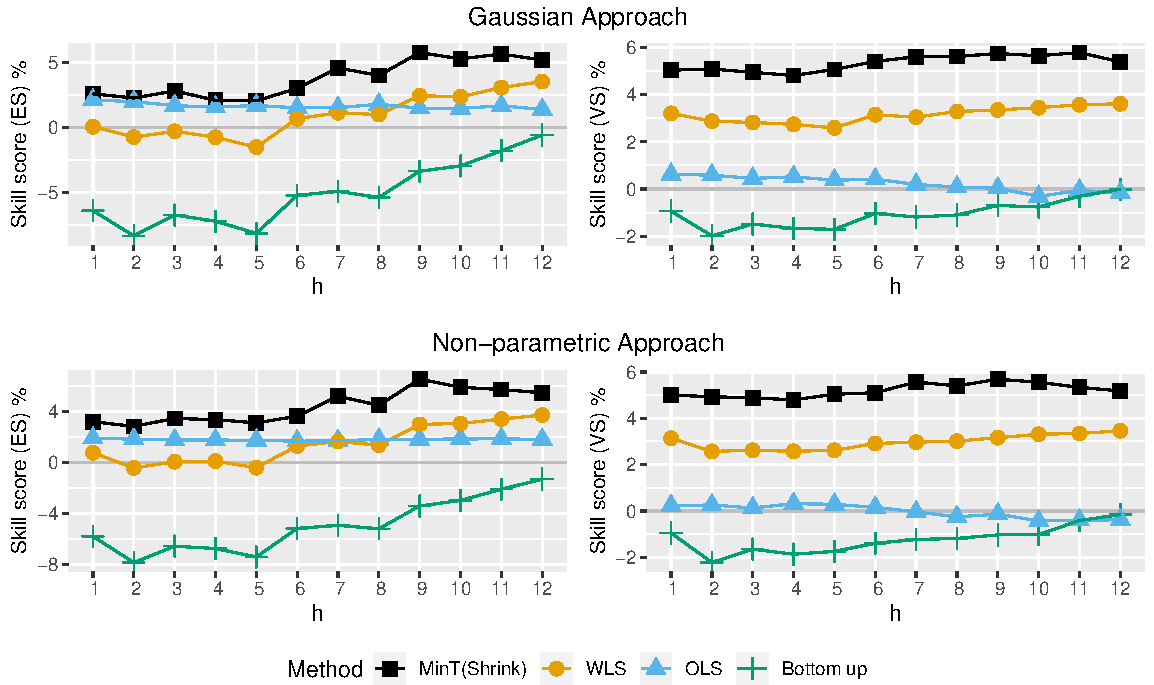
\includegraphics[width= .95\textwidth]{Empirical-results/AllTS_MultiVScores_ARIMA.pdf}
	\caption{Skill scores with reference to incoherent forecasts for multivariate predictive distribution across the entire hierarchy from different methods. A positive (negative) skill score indicates a gain (loss) in forecast accuracy over the incoherent forecast distribution. The top panel shows the results from the Gaussian approach where the bottom panel shows the results from the non-parametric approach. Left and right panels show the skill scores based on energy and variogram scores respectively.}\label{fig:EmpResults_AllTS}
\end{figure}

\begin{figure}
	\centering
	\small
	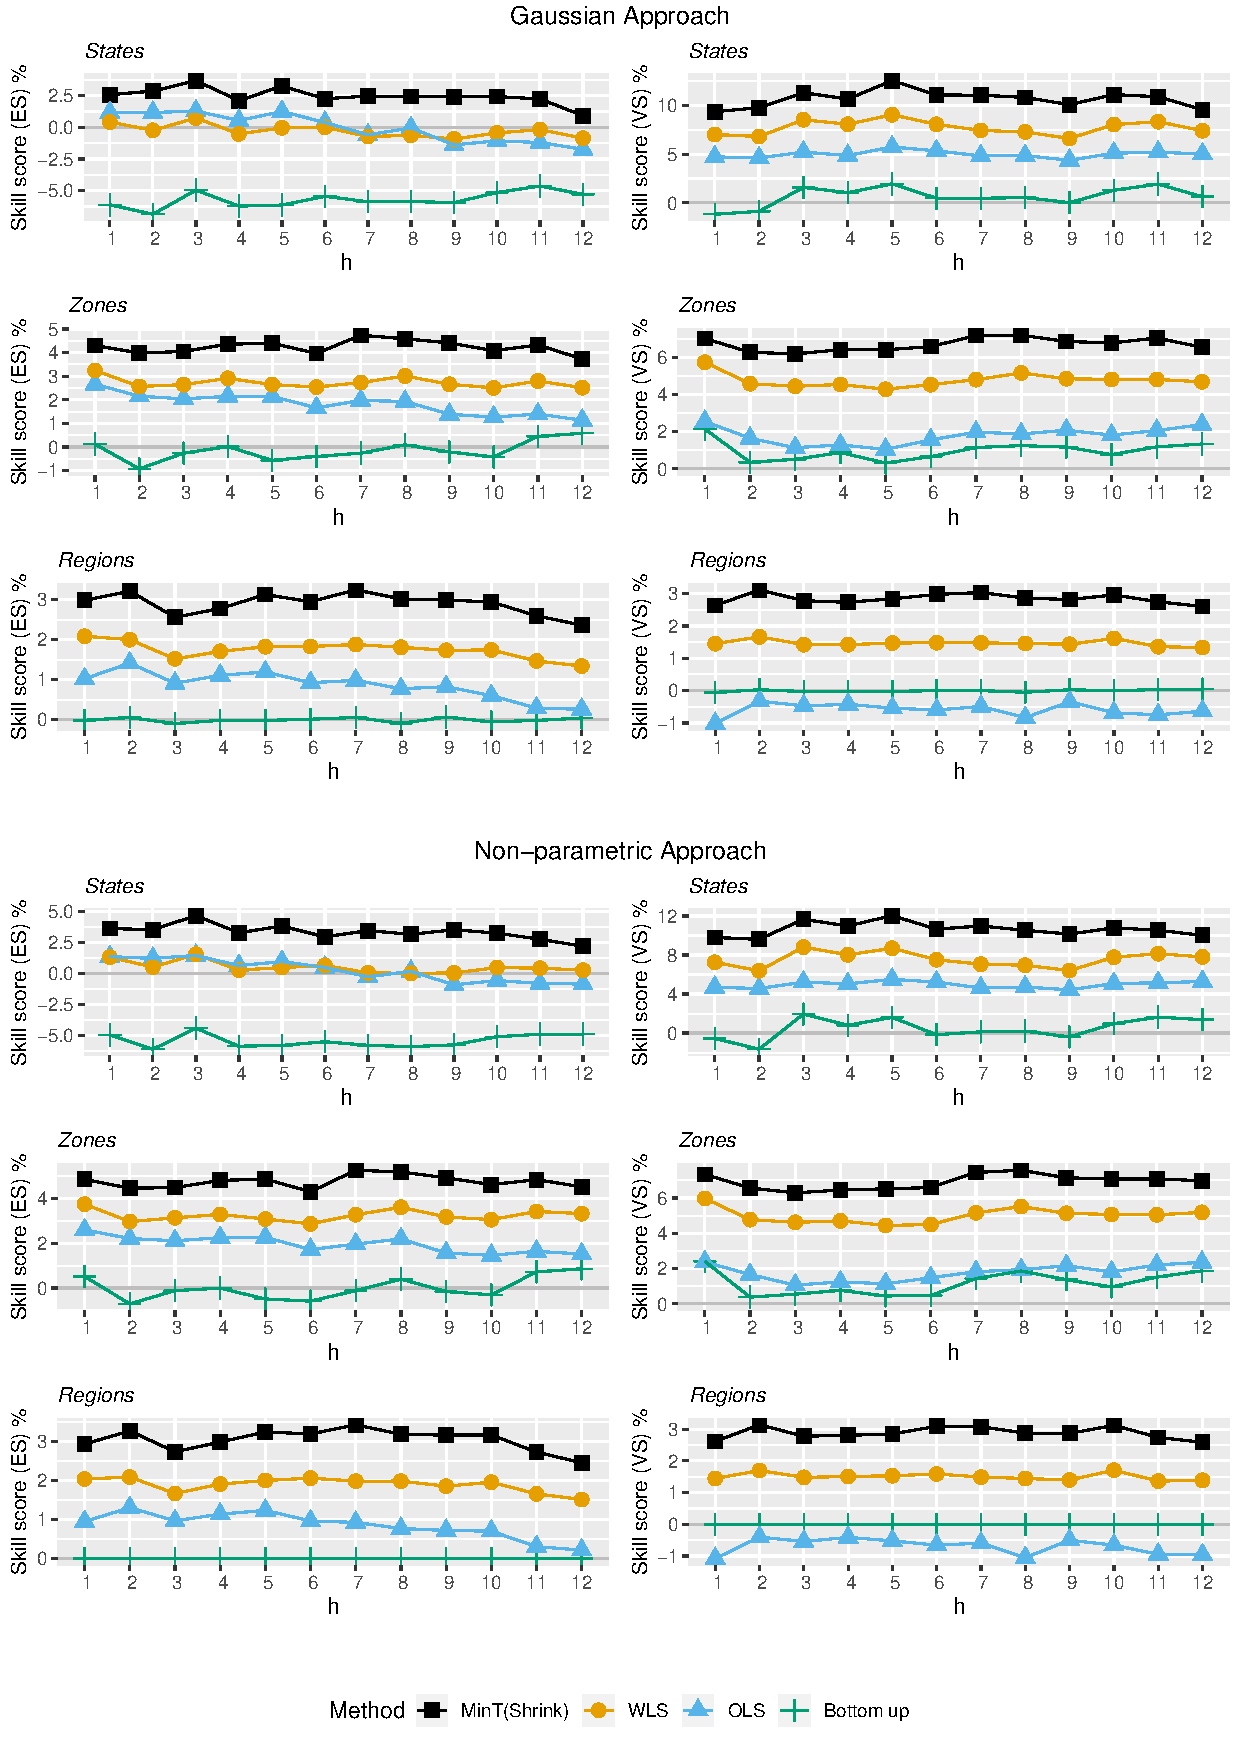
\includegraphics[width= 0.8\textwidth, height= 0.85\textheight]{Empirical-results/Levels_MultiVScores_ARIMA.pdf}
	\caption{Skill scores for multivariate probabilistic forecasts across different levels of the hierarchy. A positive (negative) skill score indicates a gain (loss) in forecast accuracy over the incoherent forecast distribution. Results from the Gaussian approach are presented in the top three panels while results from the non-parametric approach are presented in the bottom three panels.}\label{fig:EmpResults_Levels}
\end{figure}

\begin{figure}
	\centering
	\small
	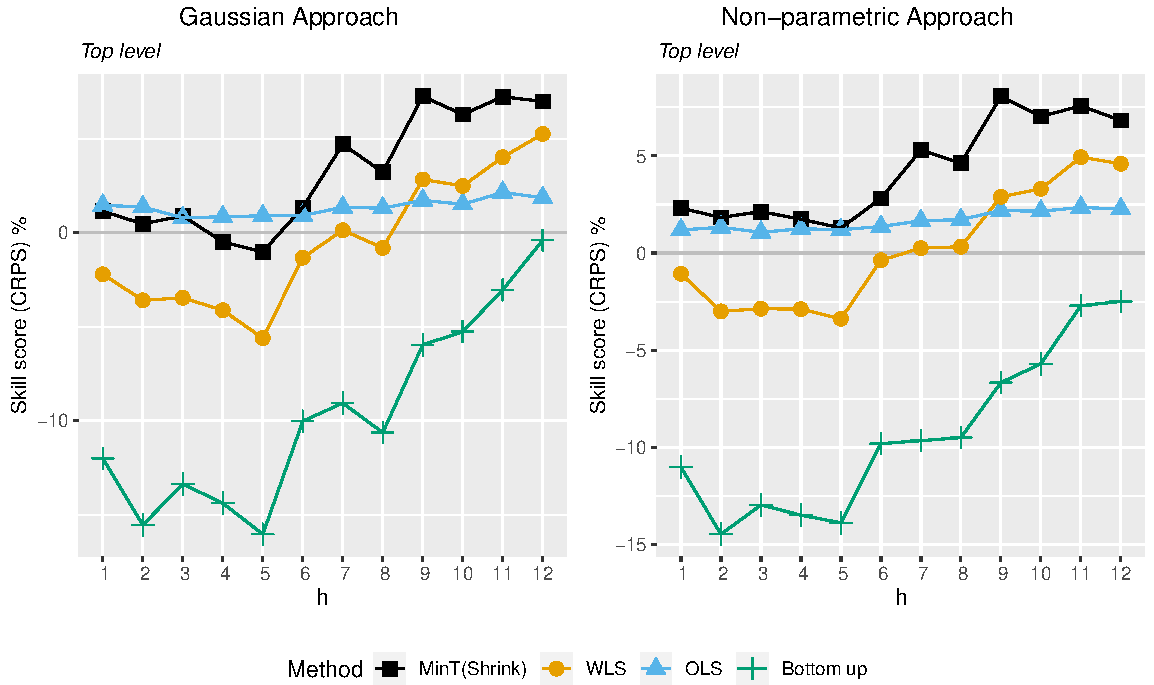
\includegraphics[width= \textwidth]{Empirical-results/UniVScore_TopLevel_ARIMA.pdf}
	\caption{Skill score based on CRPS (with reference to the incoherent forecasts) for univariate probabilistic forecasts for the Total (top level) overnight trips. A positive (negative) skill score indicates a gain (loss) in forecast accuracy over the incoherent forecast distribution. Left panel shows the results from the Gaussian approach and right panel shows the results from the non-parametric approach. }\label{fig:EmpResults_TopLevel}
\end{figure}

Figure \ref{fig:EmpResults_AllTS} shows the skill scores with respect to the multivariate predictive distributions across the entire hierarchy from the different methods. Figure \ref{fig:EmpResults_Levels} shows the evaluation across each level. The top panels present the results from the Gaussian approach while the bottom panels present the results from the non-parametric approach. Both figures show that almost all reconciliation methods improve forecast accuracy irrespective of whether the parametric or non-parametric approaches are implemented. Furthermore, the bottom-up approach shows losses compared to the incoherent forecasts at all forecast horizons. This reflects the fact that bottom-level series are noisier and therefore more challenging to forecast. Finally and most importantly, MinT(Shrink) outperforms all probabilistic forecast reconciliation methods for both parametric and non-parametric approaches.

Figure \ref{fig:EmpResults_TopLevel} shows the predictive accuracy of the univariate forecast distributions for the Total overnight trips. OLS and MinT(Shrink) reconciliation methods show gains in accuracy for the top level of the hierarchy for both Gaussian and non-parametric approaches.





\section{Conclusions}\label{sec:conclusions_chap3}

Although hierarchical point forecasting is well studied in the literature, there has been a relative lack of attention given to the probabilistic setting. We fill this gap in the literature by providing a mathematically rigorous formulation of coherence and reconciliation for probabilistic forecasts.

The geometric interpretation of point forecast reconciliation can be extended to the probabilistic setting. We have also discussed strategies for evaluating probabilistic forecasts for hierarchical time series advocating the use of multivariate scoring rules on the full hierarchy, while establishing a key result that the log score is not proper with respect to incoherent forecasts.

We have shown that for elliptical distributions the true predictive density can be recovered by linear reconciliation and we have established conditions for when this is a projection. Although this projection cannot feasibly be obtained in practice, a projection similar to the MinT approach provides a good approximation in applications. This is supported by the results of a simulation study as well as the empirical application.

We have further proposed a novel non-parametric approach for obtaining coherent probabilistic forecasts for when the parametric densities are unavailable. Initially this method involves generating thousands of sample paths using bootstrapped forecast errors. Then each sample path is reconciled via projections. Using an extensive simulation setting we have shown that the MinT projection is at least as good as the optimal projection with respect to minimising Energy score. Further we have shown in an empirical application that reconciled probabilistic forecasts via MinT show gains in the forecast accuracy over incoherent and bottom-up forecasts.


In many ways this chapter sets up a substantial future research agenda. For example, having defined what amounts to an entire class of reconciliation methods for probabilistic forecasts it will be worthwhile investigating which specific projections are optimal. This is likely to depend on the specific scoring rule employed as well as the properties of the base forecasts. Another avenue worth investigating is to consider whether it is possible to recover the true predictive distribution for non-elliptical distributions via a non-linear function $g(.)$.

\newpage

\appendix

\section{Reparameterisation of $\bm{G}$ in optimal reconciliation of future paths} \label{Appen:ReparaG}

We consider different parameterisations when estimating the optimal $\bm{G}_h$ via the proposed optimisation process. Let,
\begin{equation}\label{eq:StructureofG}
\bm{G}_h = (\bm{S'W}_h\bm{S})^{-1}\bm{S'W}_h.
\end{equation}
This structure for $\bm{G}_h$ will ensure $\bm{SG}_h$ is a projection matrix and it projects each sample path onto $\mathfrak{s}$.
\begin{itemize}
	\item[\textbf{Method 1}] Minimising the objective function in (\ref{eq:Obj_func_2}) over symmetric $\bm{W}_h$. This solves an unconstrained optimisation problem
	\item[\textbf{Method 2}] Consider the Cholesky decomposition of $\bm{W}_h$. i.e. let $\bm{W}_h = \bm{U}_h'\bm{U}_h$ where $\bm{U}_h$ is an upper triangular matrix. Thus minimising (\ref{eq:Obj_func_2}) over $\bm{U}_h$
	\item[\textbf{Method 3}] Similar to method 2, minimising (\ref{eq:Obj_func_2}) over the Cholesky decomposition of $\bm{W}_h$, but imposing restrictions for scaling. i.e., $\bm{W}_h=\bm{U}_h'\bm{U}_h \quad \text{s.t} \quad \bm{i'}\bm{W}_h\bm{i}=1$ where $\bm{i}=(1,0,..,0)'$
	\item[\textbf{Method 4}] Minimising (\ref{eq:Obj_func_2}) over $\bm{G}_h$ such that $\bm{G}_h\bm{S}=\bm{I}$. This constraint is an alternative way to ensure that $\bm{SG}_h$ is a projection onto $\mathfrak{s}$
	
\end{itemize}

\section{Simulations}

\subsection{Imposing higher signal-to-noise ratio in aggregate levels}\label{Append:sig-to-noise}

In practice, hierarchical time series are likely to have relatively noisier series at lower levels of aggregation. Following the method proposed by \citet{WicEtAl2019}, we replicate this feature in our simulations by generating the bottom-level series $\{y_{AA,t},y_{AB,t},y_{BA,t},y_{BB,t}\}$ as follows:
\begin{align*}
y_{AA,t} &= w_{AA,t} + u_t - 0.5v_t,\\
y_{AB,t} &= w_{AB,t} - u_t - 0.5v_t,\\
y_{BA,t} &= w_{BA,t} + u_t + 0.5v_t,\\
y_{BB,t} &= w_{BB,t} - u_t + 0.5v_t,
\end{align*}
where $u_t \sim \mathcal{N}(0,\sigma^2_u)$ and $v_t \sim \mathcal{N}(0,\sigma^2_v)$. The aggregate series in the middle-level are given by:
\begin{align*}
y_{A,t} &= w_{AA,t} + w_{AB,t} - v_t,\\
y_{B,t} &= w_{BA,t} + w_{BB,t} + v_t,
\end{align*}
and the total series is given by
\[
y_{Tot,t} = w_{AA,t} + w_{AB,t} + w_{BA,t} + w_{BB,t}.
\]


To ensure the disaggregate series are noisier than the aggregate series, we choose $\sigma^2_u$ and $\sigma^2_v$ such that
\[
\var(\varepsilon_{AA,t} + \varepsilon_{AB,t} + \varepsilon_{BA,t} + \varepsilon_{BB,t})
\le \var(\varepsilon_{AA,t}+\varepsilon_{AB,t}-v_t)
\le \var(\varepsilon_{AA,t}+u_t-0.5v_t).
\]
Similar inequalities hold when $\varepsilon_{AA,t}$ is replaced by $\varepsilon_{AB,t}$, $\varepsilon_{BA,t}$ and $\varepsilon_{BB,t}$ in the third term.

Thus for the Gaussian DGP we choose $\sigma^2_u = 24$ and $\sigma^2_u = 18$ whereas for non-Gaussian DGP we choose $\sigma^2_u = 10$ and $\sigma^2_v = 7$.

\subsection{Simulation results from parametric solution for marginal forecast distributions}\label{Append:Gauss_sim_Univ}

\begin{table}[H]
	\caption{Comparison of incoherent vs coherent forecasts based on the univariate forecast distribution of the aggregate series. Each entry represents the percentage skill score with reference to the incoherent forecasts based on ``CRPS" and ``LS". These entries show the percentage increase in score for different forecasting methods relative to the incoherent forecasts for $h=2$ and $3$ steps-ahead forecast. Results from the Gaussian DGP are presented in the top panel whereas the results from the non-Gaussian DGP are presented in the bottom panel}\label{tab:SimResults_Gauss_UnivScores_Aggre_h2-h3}
	\centering
	\resizebox{\linewidth}{!}{
		\begin{tabular}{lcccccccccccc}
			\toprule
			\multicolumn{1}{c}{ } & \multicolumn{6}{c}{h=2} &
			\multicolumn{6}{c}{h=3} \\
			\cmidrule(lr){2-7} \cmidrule(lr){8-13}
			\multicolumn{1}{c}{ } & \multicolumn{2}{c}{Total} & \multicolumn{2}{c}{A} & \multicolumn{2}{c}{B} & \multicolumn{2}{c}{Total} & \multicolumn{2}{c}{A} & \multicolumn{2}{c}{B} \\
			\cmidrule(lr){2-3} \cmidrule(lr){4-5} \cmidrule(lr){6-7} \cmidrule(lr){8-9} \cmidrule(lr){10-11} \cmidrule(lr){12-13} 
			
			R.method & CRPS & LS & CRPS & LS & CRPS & LS & CRPS & LS & CRPS & LS & CRPS & LS\\
			\toprule
			\multicolumn{13}{c}{Gaussian DGP}\\
			\toprule
			
			MinT(Shrink) & \textbf{0.34} & -0.08 & 10.67 & 3.32 & 5.79 & 1.59 & 0.08 & -0.17 & 8.13 & 1.58 & 4.17 & 1.04\\
			
			MinT(Sample) & 0.27 & -0.10 & \textbf{10.76} & \textbf{3.39} & 5.67 & 1.62 & 0.04 & -0.23 & \textbf{8.14} & \textbf{1.69} & 4.19 & 1.10\\
			
			WLS & -0.41 & 1.02 & 9.99 & 2.97 & \textbf{6.01} & \textbf{1.73} & \textbf{0.10} & 2.97 & 7.72 & 1.57 & \textbf{4.46} & 1.26\\
			
			OLS & -5.99 & \textbf{4.05} & 7.17 & 2.03 & 5.83 & 1.70 & -2.13 & 13.11 & 5.30 & 0.97 & 4.41 & \textbf{1.30}\\
			
			Bottom up & -60.07 & 2.72 & -13.82 & -3.86 & -9.04 & -2.37 & -30.95 & \textbf{30.34} & -13.57 & -3.37 & -8.47 & -1.87\\
			
			Incoherent & 0.00 & 0.00 & 0.00 & 0.00 & 0.00 & 0.00 & 0.00 & 0.00 & 0.00 & 0.00 & 0.00 & 0.00\\
			
			\toprule
			\multicolumn{13}{c}{Non-Gaussian DGP}\\
			\toprule
			
			MinT(Shrink) & -0.70 & -1.16 & \textbf{0.71} & 0.29 & \textbf{16.53} & 6.83 & -0.30 & -1.35 & \textbf{0.60} & 0.25 & \textbf{19.53} & 8.28\\
			
			MinT(Sample) & -0.70 & -1.53 & \textbf{0.71} & \textbf{0.31} & \textbf{16.53} & \textbf{6.87} & -0.30 & -1.61 & \textbf{0.60} & \textbf{0.31} & \textbf{19.53} & \textbf{8.35}\\
			
			WLS & -0.11 & -0.15 & -2.50 & -1.09 & 13.87 & 5.55 & -0.02 & -0.40 & -3.96 & -1.60 & 16.14 & 6.78\\
			
			OLS & -44.06 & -14.27 & -0.18 & -0.12 & 8.72 & 3.44 & -22.75 & \textbf{19.51} & -0.71 & -0.32 & 10.48 & 4.27\\
			
			Bottom up & -273.80 & -68.47 & -4.20 & -1.67 & -8.78 & -2.84 & -159.47 & 10.59 & -4.71 & -1.77 & -8.06 & -2.27\\
			
			Incoherent & 0.00 & 0.00 & 0.00 & 0.00 & 0.00 & 0.00 & 0.00 & 0.00 & 0.00 & 0.00 & 0.00 & 0.00\\
			\bottomrule
		\end{tabular}
	}
\end{table}



\begin{table}[H]
	\caption{Comparison of incoherent vs coherent forecasts based univariate forecast distribution of bottom-level series. Each entry represents the skill score with reference to Incoherent forecasts based on ``CRPS" and ``LS" for forecast horizons $h=2$ and $h=3$.}\label{tab:SimResults_Gauss_UnivScores_Disaggre_h2-h3}
	\centering
	\resizebox{\linewidth}{!}{
		\begin{tabular}{lcccccccccccccccc}
			\toprule
			\multicolumn{1}{c}{ } & \multicolumn{8}{c}{h=2} &
			\multicolumn{8}{c}{h=3} \\
			\cmidrule(lr){2-9} \cmidrule(lr){10-17}
			\multicolumn{1}{c}{ } & \multicolumn{2}{c}{AA} & \multicolumn{2}{c}{AB} & \multicolumn{2}{c}{BA} & \multicolumn{2}{c}{BB} & \multicolumn{2}{c}{AA} & \multicolumn{2}{c}{AB} & \multicolumn{2}{c}{BA} & \multicolumn{2}{c}{BB} \\
			\cmidrule(lr){2-3} \cmidrule(lr){4-5} \cmidrule(lr){6-7} \cmidrule(lr){8-9} \cmidrule(lr){10-11} \cmidrule(lr){12-13} \cmidrule(lr){14-15} \cmidrule(lr){16-17} 
			R.method & CRPS & LS & CRPS & LS & CRPS & LS & CRPS & LS & CRPS & LS & CRPS & LS & CRPS & LS & CRPS & LS\\
			\toprule
			\multicolumn{17}{c}{Gaussian DGP}\\
			\toprule
			
			MinT(Shrink) & 3.80 & 1.28 & \textbf{19.37} & \textbf{6.55} & \textbf{13.61} & \textbf{4.44} & -0.08 & -0.14 & \textbf{2.54} & \textbf{0.83} & \textbf{19.58} & \textbf{6.92} & \textbf{13.94} & \textbf{4.83} & -2.64 & -0.96\\
			
			MinT(Sample) & \textbf{4.06} & \textbf{1.33} & 19.23 & 6.53 & 13.21 & 4.34 & -0.24 & -0.19 & 2.24 & 0.68 & 19.33 & 6.73 & 13.44 & 4.62 & -3.44 & -1.21\\
			
			WLS & -0.55 & -0.09 & 15.52 & 5.05 & 12.17 & 3.91 & -3.48 & -1.25 & -1.52 & -0.46 & 15.75 & 5.32 & 12.63 & 4.34 & -5.74 & -2.04\\
			
			OLS & -1.23 & -0.30 & 12.09 & 3.83 & 10.19 & 3.25 & -4.42 & -1.57 & -2.04 & -0.60 & 11.96 & 3.93 & 10.44 & 3.45 & -6.72 & -2.36\\
			
			Bottom up & -0.01 & 0.00 & 0.17 & -0.01 & 0.12 & 0.00 & \textbf{0.17} & 0.00 & -0.23 & 0.00 & -0.01 & -0.02 & 0.01 & -0.01 & -0.13 & 0.00\\
			
			Base & 0.00 & 0.00 & 0.00 & 0.00 & 0.00 & 0.00 & 0.00 & 0.00 & 0.00 & 0.00 & 0.00 & 0.00 & 0.00 & 0.00 & 0.00 & 0.00\\
			\toprule
			\multicolumn{17}{c}{Non-Gaussian DGP}\\
			\toprule
			
			MinT(Shrink) & \textbf{3.67} & \textbf{1.30} & -0.11 & -0.18 & \textbf{16.19} & \textbf{6.12} & \textbf{2.29} & \textbf{0.80} & 3.38 & 1.22 & -1.21 & -0.47 & \textbf{17.90} & \textbf{6.92} & \textbf{2.09} & \textbf{0.76}\\
			
			MinT(Sample) & \textbf{3.67} & 1.25 & -0.11 & -0.24 & \textbf{16.19} & 6.01 & \textbf{2.29} & 0.76 & 3.38 & 1.16 & -1.21 & -0.58 & \textbf{17.90} & 6.71 & \textbf{2.09} & 0.64\\
			
			WLS & 3.34 & 1.24 & -2.51 & -1.00 & 10.79 & 3.96 & -1.27 & -0.38 & \textbf{3.47} & \textbf{1.23} & -3.11 & -1.12 & 12.60 & 4.78 & -1.21 & -0.41\\
			
			OLS & 2.95 & 1.15 & -1.85 & -0.73 & 7.61 & 2.74 & -1.19 & -0.32 & 3.22 & 1.18 & -2.13 & -0.76 & 8.85 & 3.25 & -1.13 & -0.35\\
			
			Bottom up & -0.17 & 0.00 & 0.09 & 0.00 & 0.03 & -0.01 & -0.10 & 0.00 & -0.20 & 0.00 & -0.03 & 0.00 & -0.05 & -0.01 & -0.22 & 0.00\\
			
			Base & 0.00 & 0.00 & 0.00 & 0.00 & 0.00 & 0.00 & 0.00 & 0.00 & 0.00 & 0.00 & 0.00 & 0.00 & 0.00 & 0.00 & 0.00 & 0.00\\
			\bottomrule
		\end{tabular}
	}
\end{table}



\subsection{Simulation results from the comparison of different re-parameterisation methods for $\bm{G}$}\label{Appen:ReparaG_sim}

\begin{table}
	\caption{Energy scores (ES) and variogram scores (VS) for reconciled probabilistic forecasts from different parameterisation methods are presented.} \label{table:Non-paraSim_re-para}
	%	\centering
	\begin{center}
		\tabcolsep=0.08cm\small
		\resizebox{\linewidth}{!}{
			\begin{tabular}{@{}lSSSSSS|SSSSSS@{}}
				\toprule
				\multicolumn{1}{c}{} & \multicolumn{6}{c|}{Non-Gaussian DGP} & \multicolumn{6}{c}{Gaussian DGP}\\
				\toprule
				Reconciliation &
				\multicolumn{2}{c}{h=1} &
				\multicolumn{2}{c}{h=2} &
				\multicolumn{2}{c|}{h=3} & \multicolumn{2}{c}{h=1} &
				\multicolumn{2}{c}{h=2} &
				\multicolumn{2}{c}{h=3} \\
				\cmidrule(lr){2-3} \cmidrule(lr){4-5} \cmidrule(lr){6-7} \cmidrule(lr){8-9} \cmidrule(lr){10-11} \cmidrule(lr){12-13}
				method       & {}{\text{ES}} &  {\text{VS}} & {\text{ES}} &  {\text{VS}} & {\text{ES}} &  {\text{VS}} &{\text{ES}} &  {\text{VS}} & {\text{ES}} &  {\text{VS}} & {\text{ES}} &  {\text{VS}} \\
				\midrule
				Optimal(Method-1) & 5.36 & 1.21 & 5.51 & 1.27 & 5.83 & 1.38 & 9.59 & 4.86 & 11.50 & 5.38 & 13.80 & 6.13\\
				Optimal(Method-2) & 5.37 & 1.21 & 5.53 & 1.27 & 5.83 & 1.37 & 9.58 & 4.85 & 11.50 & 5.37 & 13.80 & 6.14\\
				Optimal(Method-3) & 5.37 & 1.21 & 5.53 & 1.27 & 5.83 & 1.37 & 9.58 & 4.85 & 11.50 & 5.37 &
				13.80 & 6.14 \\
				Optimal(Method-4) & 5.38 & 1.21 & 5.54 & 1.27 & 5.83 & 1.38 & 9.58 & 4.85 & 11.50 & 5.37 & 13.80 & 6.14\\
%				MinT(Shrink)*	  & 5.33 & 1.19 & 5.50 & 1.26 & 5.77 & 1.34 & 9.43 & 4.78 & 11.40 & 5.33 & 13.70 & 6.09 \\
%				WLS          	  & 5.43 & 1.23 & 5.60 & 1.30 & 5.89 & 1.40 & 9.64 & 4.93 & 11.70 & 5.60 & 14.10 & 6.39 \\
%				OLS          	  & 5.51 & 1.23 & 5.70 & 1.30 & 5.98 & 1.40 & 9.91 & 4.93 & 12.10 & 5.60 &
%				14.50 & 6.39\\
%				\textit{Incoherent} & $\mathbi{5.71}$ & $\mathbi{1.28}$ & $\mathbi{5.94}$ & $\mathbi{1.37}$ & $\mathbi{6.27}$ & $\mathbi{1.49}$ &$\mathbi{10.40}$& $\mathbi{5.31}$ & $\mathbi{12.70}$ & $\mathbi{6.22}$ & $\mathbi{15.20}$ & $\mathbi{7.14}$\\
				\bottomrule
			\end{tabular}
		}
	\end{center}
%	\textit{The differences in scores between methods noted by ``*'' are statistically insignificant. The differences between these and the incoherent forecasts are statistically significant.}
\end{table}

\section{Application}

\subsection{Results from ETS base forecasts}

\begin{figure}[!hbt]
	\centering
	\small
	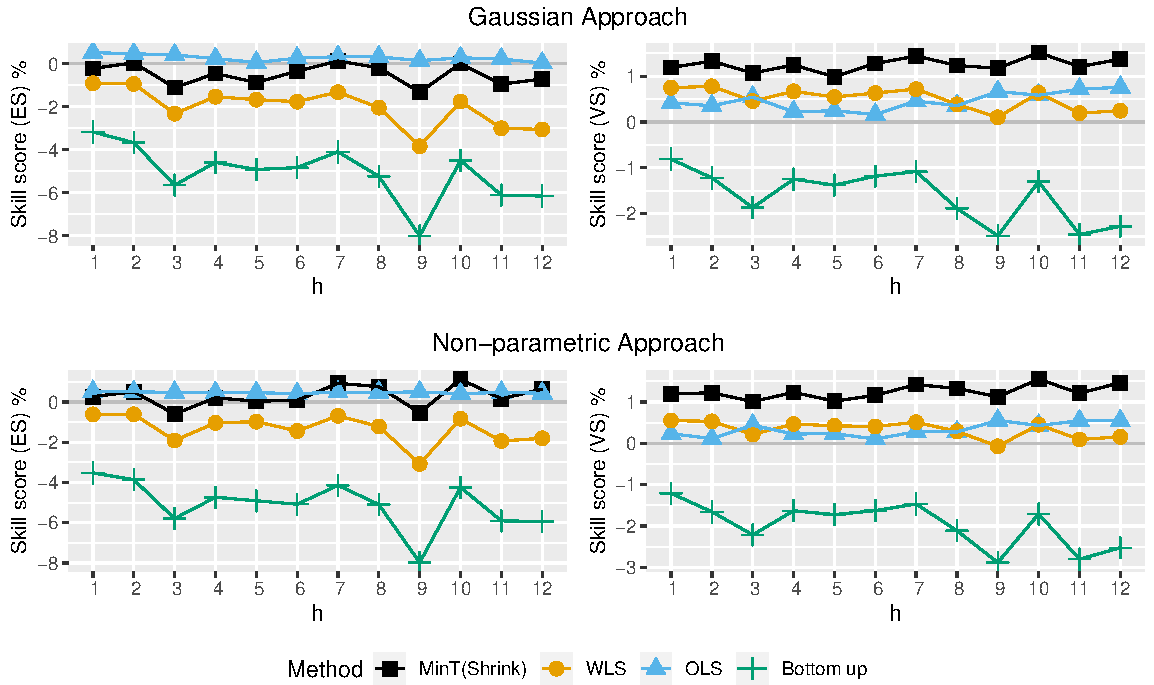
\includegraphics[width= .95\textwidth]{Empirical-results/AllTS_MultiVScores_ETS.pdf}
	\caption{Skill scores with reference to ETS base forecasts for multivariate predictive distribution of the whole hierarchy from different reconciliation methods are presented. Top panel shows the results from Gaussian approach and the bottom panel shows the results from non-parametric approach. Left and right panels shows the skill scores based on energy score and variogram score respectively.}\label{fig:EmpResults_AllTS_ETS}
\end{figure}

\begin{figure}[!hbt]
	\centering
	\small
	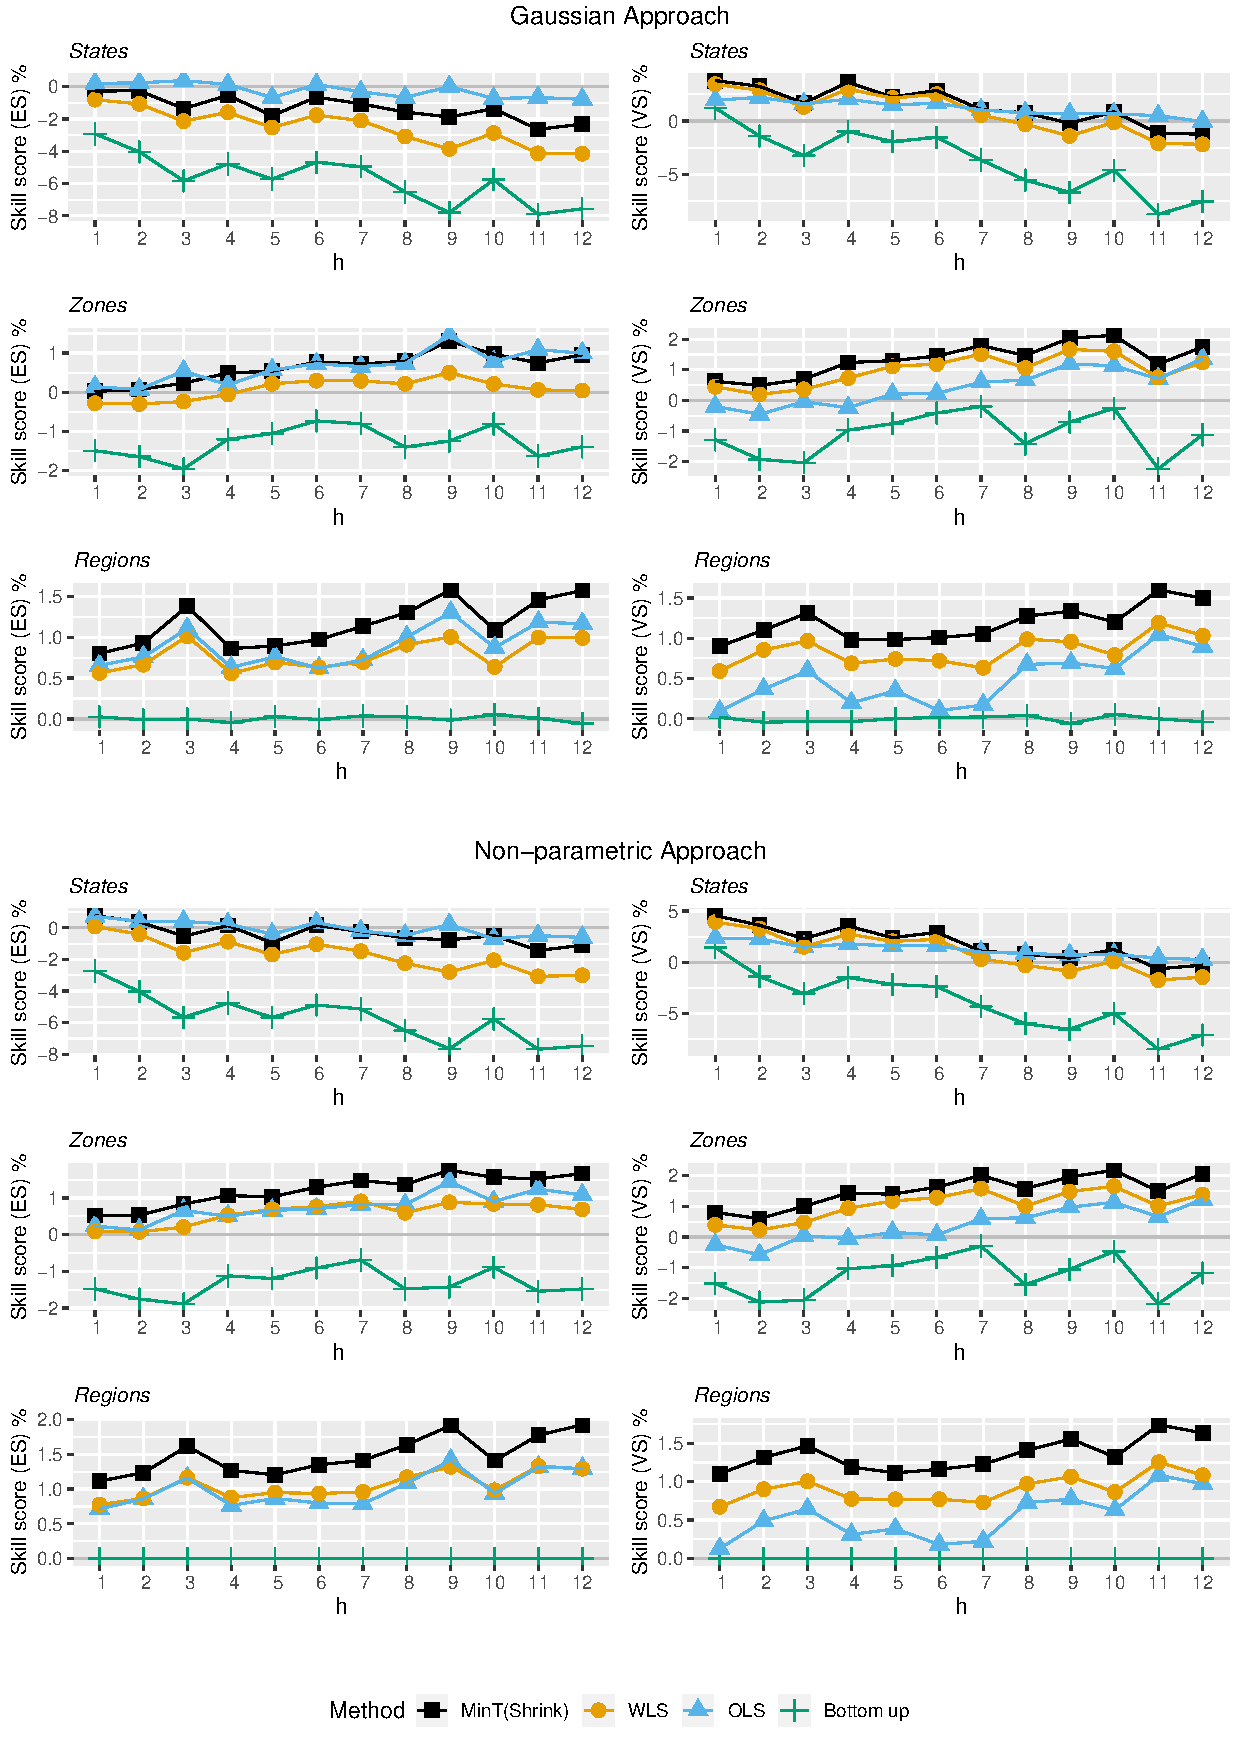
\includegraphics[width= 0.8\textwidth, height= 0.85\textheight]{Empirical-results/Levels_MultiVScores_ETS.pdf}
	\caption{Skill score (with reference to ETS base forecasts) for multivariate probabilistic forecasts of different levels of the hierarchy are presented. Results from Gaussian approach are presented in the top three panels and results from the non-parametric approach are presented in the bottom three panels.}\label{fig:EmpResults_Levels_ETS}
\end{figure}

\begin{figure}[!hbt]
	\centering
	\small
	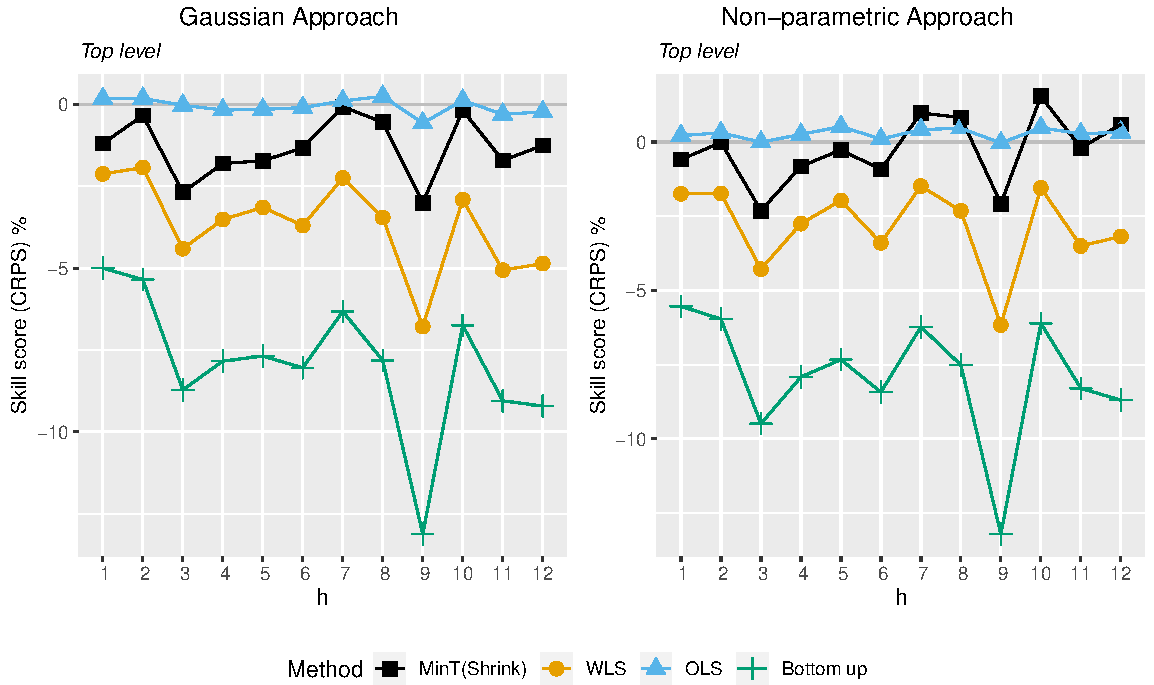
\includegraphics[width= \textwidth]{Empirical-results/UniVScore_TopLevel_ETS.pdf}
	\caption{Skill score based on CRPS (with reference to the ETS base forecasts) for univariate probabilistic forecasts for the Total (top level) overnight trips are presented. Left panel shows the results from Gaussian approach and right panel shows the results from non-parametric approach. }\label{fig:EmpResults_TopLevel_ETS}
\end{figure}

\FloatBarrier

\newpage
\subsection{Australian Tourism Data}

\begin{table}[!hb]
	\caption{Geographic hierarchy of Australian tourism flow}\label{table:A1_chap3}
	\centering\tabcolsep=0.08cm
	\fontsize{7}{7}\selectfont
	\resizebox{\linewidth}{!}{
		\begin{tabular}{lllllllllll}
			\toprule
			\multicolumn{3}{c}{\textbf{Level 0 - Total}}    &&  \multicolumn{3}{l}{\textit{Regions cont.}}   &  & \multicolumn{3}{l}{\textit{Regions cont.}} \\
			\cmidrule(lr){1-3}
			1 & {\text{Tot}} & {Australia} &&  37	& AAB & Central Coast && 75  & CBD & Mackay   \\
			\cmidrule(lr){1-3}
			\multicolumn{3}{c}{\textbf{Level 1 - States}} && 38  & ABA & Hunter && 76 & CBE & Capricorn \\
			\cmidrule(lr){1-3}
			2 & A & NSW 				&  & 39  & ABB & North Coast NSW   && 77 & CBF & Gladstone\\
			3 & B & Victoria 			&  & 40  & ACA & South Coast  && 78  & CCA & Whitsundays\\
			4 & C & Queensland 			&  & 41  & ADA & Snowy Mountains && 79  & CCB & Townsville  \\
			5 & D & South Australia     &  & 42  & ADB & Capital Country && 80  & CCC & Tropical North Queensland   \\
			6 & E & Western Australia   &  & 43  & ADC & The Murray   && 81  & CDA & Southern QLD country\\
			7 & F & Tasmania   			&  & 44  & ADD & Riverina  &&82  & CDB & Outback QLD\\
			8 & G & Northern Territory  &  & 45  & AEA & Central NSW &&83  & DAA & Adelaide   \\
			\cmidrule(lr){1-3}
			\multicolumn{3}{c}{\textbf{Level 2 - Zones}}  &  &  46  & AEB & New England North West && 84  & DAB & Barossa\\
			\cmidrule(lr){1-3}
			9 	& AA & Metro NSW 	  	   	&  & 47  & AEC & Outback NSW   &&85  & DAC & Adelaide Hills\\
			10 	& AB & North Coast NSW 	   	&  & 48  & AED & Blue Mountains  && 86  & DBA & Limestone Coast\\
			11	& AC & South Coast NSW	   	&  & 49  & AFA & Canberra   &&  87  & DBB & Fleurieu Peninsula\\
			12	& AD & South NSW 			&  & 50  & BAA & Melbourne &&88  & DBC & Kangaroo Island\\
			13	& AE & North NSW 			&  & 51  & BAB & Peninsula    &&89  & DCA & Murraylands\\
			14	& AF & ACT					&  &  52  & BAC & Geelong  && 90  & DCB & Riverland\\
			15	& BA & Metro VIC			&  &  53  & BBA & Western   &&91  & DCC & Clare Valley\\
			16	& BB & West Coast VIC		&  &  54  & BCA & Lakes  &&92  & DCD & Flinders Range and Outback\\
			17	& BC & East Coast VIC		&  &  55  & BCB & Gippsland    &&93  & DDA & Eyre Peninsula\\
			18	& BD & North East VIC		&  &  56  & BCC & Phillip Island   &&  94  & DDB & Yorke Peninsula \\
			19	& BE & North West VIC		&  &  57  & BDA & Central Murray    &&95  & EAA & Australia's Coral Coast\\
			20  & CA & Metro QLD			&  & 58  & BDB & Goulburn    &&96  & EAB & Experience Perth\\
			21  & CB & Central Coast QLD	&  & 59  & BDC & High Country   &&97  & EAC & Australia's South West\\
			22  & CC & North Coast QLD		&  &  60  & BDD & Melbourne East &&98  & EBA & Australia's North West \\
			23  & CD & Inland QLD			&  &   61  & BDE & Upper Yarra &&99  & ECA & Australia's Golden Outback\\
			24	& DA & Metro SA				&  & 62  & BDF & Murray East  && 100 & FAA & Hobart and South\\
			25	& DB & South Coast SA		&  &  63  & BEA & Wimmera+Mallee &&101 & FBA & East Coast\\
			26	& DC & Inland SA			&  & 64  & BEB & Western Grampians &&102 & FBB & Launceston, Tamar \& North\\
			27	& DD & West Coast SA		&  &65  & BEC & Bendigo Loddon  &&103 & FCA & North West\\
			
			28	& EA & West Coast WA 	& &  66  & BED & Macedon    &&104 & FCB& West coast\\
			29	& EB & North WA			& &  67  & BEE & Spa Country   &&105 & GAA& Darwin \\
			30	& EC & South WA 		& &   68  & BEF & Ballarat     &&106 & GAB& Litchfield Kakadu Arnhem\\
			31	& FA & South TAS		& &  69  & BEG & Central Highlands  &&107 & GAC& Katherine Daly\\
			32	& FB & North East TAS	& & 70  & CAA & Gold Coast  &&108 & GBA& Barkly\\
			33	& FC & North West TAS	& & 71  & CAB & Brisbane  &&109 & GBB& Lasseter\\
			34	& GA & North Coast NT	& & 72  & CAC & Sunshine Coast &&110 & GBC& Alice Springs\\
			35	& GB & Central NT		& &  73  & CBB & Bundaberg      &&111 & GBD& MacDonnell\\
			\cmidrule(lr){1-3}
			\multicolumn{3}{c}{\textbf{Level 2 - Regions}} & & 74  & CBC & Fraser Coast    &&\\
			\cmidrule(lr){1-3}
			36	& AAA & Sydney 			& 	&  &&\\
			
			\bottomrule
		\end{tabular}
	}
\end{table}

\bibliographystyle{agsm}

\bibliography{References_paper2}

\end{document}